\documentclass[bfivepaper,twosided,justified,nobib]{tufte-book}

\hypersetup{colorlinks}% uncomment this line if you prefer colored hyperlinks (e.g., for onscreen viewing)

%%
% Book metadata
\title{How I Learned to \\ Worry Productively about AI: \\  \\ Robot Apocalypses \\ Averted}
\author{Z. Irene Ying and Jordan Boyd-Graber}
\publisher{University of Maryland}

%%
% If they're installed, use Bergamo and Chantilly from www.fontsite.com.
% They're clones of Bembo and Gill Sans, respectively.
%\IfFileExists{bergamo.sty}{\usepackage[osf]{bergamo}}{}% Bembo
%\IfFileExists{chantill.sty}{\usepackage{chantill}}{}% Gill Sans

%\usepackage{microtype}

\usepackage{booktabs}
\usepackage{graphicx}
\setkeys{Gin}{width=\linewidth,totalheight=\textheight,keepaspectratio}
\graphicspath{{figures/}}

% The fancyvrb package lets us customize the formatting of verbatim
% environments.  We use a slightly smaller font.
\usepackage{fancyvrb}
\fvset{fontsize=\normalsize}

%%
% Prints a trailing space in a smart way.
\usepackage{xspace}

\newif\ifcomment\commentfalse


\newcommand{\TL}{Tufte-\LaTeX\xspace}

% Prints the month name (e.g., January) and the year (e.g., 2008)
\newcommand{\monthyear}{%
  \ifcase\month\or January\or February\or March\or April\or May\or June\or
  July\or August\or September\or October\or November\or
  December\fi\space\number\year
}


% Prints an epigraph and speaker in sans serif, all-caps type.
\newcommand{\openepigraph}[2]{%
  %\sffamily\fontsize{14}{16}\selectfont
  \begin{fullwidth}
  \sffamily\large
  \begin{doublespace}
  \noindent\allcaps{#1}\\% epigraph
  \noindent\allcaps{#2}% author
  \end{doublespace}
  \end{fullwidth}
}

% Inserts a blank page


\newcommand{\movie}[1]{\textit{#1}}
\newcommand{\episode}[1]{``#1''}
\newcommand{\song}[1]{``#1''}
\newcommand{\series}[1]{\textit{#1}}
\newcommand{\book}[1]{\textit{#1}}


\newcommand{\sectionBreak}{\par\noindent\rule{\textwidth}{0.4pt}}
\newcommand{\quoted}[2]{\begin{quote}
    #1
  \end{quote}
  \begin{flushright}
    -- #2
  \end{flushright}
}


\newcommand{\abr}[1]{\textsc{#1}}

% Macros for typesetting the documentation
\newcommand{\hlred}[1]{\textcolor{Maroon}{#1}}% prints in red
\newcommand{\hangleft}[1]{\makebox[0pt][r]{#1}}
\newcommand{\hairsp}{\hspace{1pt}}% hair space
\newcommand{\hquad}{\hskip0.5em\relax}% half quad space
\newcommand{\TODO}[1]{\textcolor{red}{\bf TODO: #1}\xspace}
\newcommand{\na}{\quad--}% used in tables for N/A cells
\providecommand{\XeLaTeX}{X\lower.5ex\hbox{\kern-0.15em\reflectbox{E}}\kern-0.1em\LaTeX}
\newcommand{\tXeLaTeX}{\XeLaTeX\index{XeLaTeX@\protect\XeLaTeX}}
% \index{\texttt{\textbackslash xyz}@\hangleft{\texttt{\textbackslash}}\texttt{xyz}}
\newcommand{\tuftebs}{\symbol{'134}}% a backslash in tt type in OT1/T1
\newcommand{\doccmdnoindex}[2][]{\texttt{\tuftebs#2}}% command name -- adds backslash automatically (and doesn't add cmd to the index)
\newcommand{\doccmddef}[2][]{%
  \hlred{\texttt{\tuftebs#2}}\label{cmd:#2}%
  \ifthenelse{\isempty{#1}}%
    {% add the command to the index
      \index{#2 command@\protect\hangleft{\texttt{\tuftebs}}\texttt{#2}}% command name
    }%
    {% add the command and package to the index
      \index{#2 command@\protect\hangleft{\texttt{\tuftebs}}\texttt{#2} (\texttt{#1} package)}% command name
      \index{#1 package@\texttt{#1} package}\index{packages!#1@\texttt{#1}}% package name
    }%
}% command name -- adds backslash automatically
\newcommand{\doccmd}[2][]{%
  \texttt{\tuftebs#2}%
  \ifthenelse{\isempty{#1}}%
    {% add the command to the index
      \index{#2 command@\protect\hangleft{\texttt{\tuftebs}}\texttt{#2}}% command name
    }%
    {% add the command and package to the index
      \index{#2 command@\protect\hangleft{\texttt{\tuftebs}}\texttt{#2} (\texttt{#1} package)}% command name
      \index{#1 package@\texttt{#1} package}\index{packages!#1@\texttt{#1}}% package name
    }%
}% command name -- adds backslash automatically
\newcommand{\docopt}[1]{\ensuremath{\langle}\textrm{\textit{#1}}\ensuremath{\rangle}}% optional command argument
\newcommand{\docarg}[1]{\textrm{\textit{#1}}}% (required) command argument
\newenvironment{docspec}{\begin{quotation}\ttfamily\parskip0pt\parindent0pt\ignorespaces}{\end{quotation}}% command specification environment
\newcommand{\docenv}[1]{\texttt{#1}\index{#1 environment@\texttt{#1} environment}\index{environments!#1@\texttt{#1}}}% environment name
\newcommand{\docenvdef}[1]{\hlred{\texttt{#1}}\label{env:#1}\index{#1 environment@\texttt{#1} environment}\index{environments!#1@\texttt{#1}}}% environment name
\newcommand{\docpkg}[1]{\texttt{#1}\index{#1 package@\texttt{#1} package}\index{packages!#1@\texttt{#1}}}% package name
\newcommand{\doccls}[1]{\texttt{#1}}% document class name
\newcommand{\docclsopt}[1]{\texttt{#1}\index{#1 class option@\texttt{#1} class option}\index{class options!#1@\texttt{#1}}}% document class option name
\newcommand{\docclsoptdef}[1]{\hlred{\texttt{#1}}\label{clsopt:#1}\index{#1 class option@\texttt{#1} class option}\index{class options!#1@\texttt{#1}}}% document class option name defined
\newcommand{\docmsg}[2]{\bigskip\begin{fullwidth}\noindent\ttfamily#1\end{fullwidth}\medskip\par\noindent#2}
\newcommand{\docfilehook}[2]{\texttt{#1}\index{file hooks!#2}\index{#1@\texttt{#1}}}
\newcommand{\doccounter}[1]{\texttt{#1}\index{#1 counter@\texttt{#1} counter}}


% \ExecuteBibliographyOptions{doi=false}
% \newbibmacro{string+doi}[1]{%
%   \iffieldundef{doi}{#1}{\href{http://dx.doi.org/\thefield{doi}}{#1}}}
% \DeclareFieldFormat{title}{\usebibmacro{string+doi}{\mkbibemph{#1}}}
% \DeclareFieldFormat[article]{title}{\usebibmacro{string+doi}{\mkbibquote{#1}}}


% Generates the index
\usepackage{makeidx}
\usepackage{natbib}
\setcitestyle{authoryear}

\makeindex
\newcommand{\blankpage}{\newpage\hbox{}\thispagestyle{empty}\newpage}
\begin{document}

% Front matter

\frontmatter




\jbgcomment{The character names should be understandable through the
  whole book.  ``Boss'' only makes sense in the first chapter.  You
  also don't use the macro consistently.  There are ReVOLTlutions and
  whatnot in your chapter.  For this to work, they must be used
  consistently.}

\newcommand{\protag}{Susan}
\newcommand{\sidetag}{Calvin}
\newcommand{\lastname}{Hobbes}

% Energy Story
\newcommand{\energyCompany}{ReVOLTlution}
\newcommand{\energyJerk}{Canyon}
\newcommand{\crunchyCity}{Bayder}
\newcommand{\Boss}{Trisha}

% General AI
\newcommand{\specializedai}{Entrench}

% Finance
\newcommand{\fintech}{StockOverflow}


% r.3 full title page
\maketitle


% v.4 copyright page
\newpage
\begin{fullwidth}
~\vfill
\thispagestyle{empty}
\setlength{\parindent}{0pt}
\setlength{\parskip}{\baselineskip}
Copyright \copyright\ \the\year\ \thanklessauthor

%\par\smallcaps{Published by \thanklesspublisher}

\par\smallcaps{tufte-latex.github.io/tufte-latex/}

\par\textit{\monthyear}
\end{fullwidth}

% r.5 contents
%\tableofcontents

%\listoffigures

%\listoftables

% r.7 dedication
% \cleardoublepage
% ~\vfill
% \begin{doublespace}
% \noindent\fontsize{18}{22}\selectfont\itshape
% \nohyphenation
% Bennet is great!
% \end{doublespace}
% \vfill
% \vfill


\cleardoublepage
\chapter{Introduction: Who should fear the Robot Apocolypse}

The news and popular culture want us to fear the robot apocolypse.  Newspapers warn us that robots are coming for our jobs, and science fiction claims that the robots are coming for our lives.  At the same time, researchers building artificial intelligence are heralding their sucesses at Go~\cite{silver-16}, Starcraft~\cite{vinyals2017starcraft}, and \series{Jeopardy!}~\cite{ferruci-10} a revolution is around the corner.

\begin{marginfigure}%
  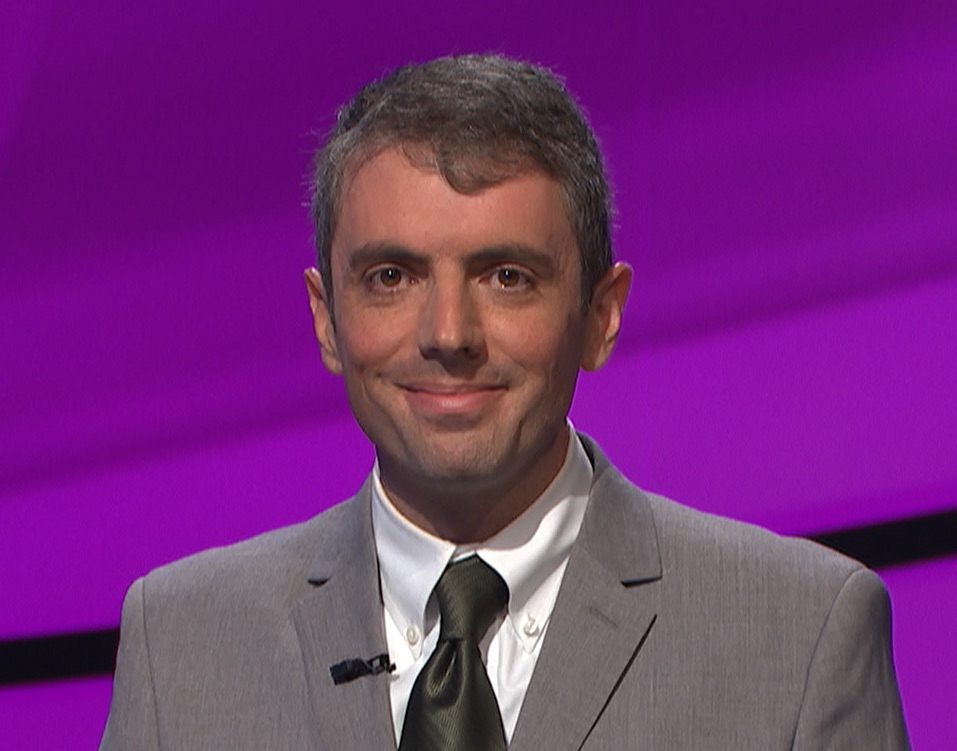
\includegraphics[width=\linewidth]{jbg}
  \caption{\href{http://boydgraber.org}{Jordan Boyd-Graber} is an associate professor at the University of Maryland who researches how computers can learn from humans and compete with humans.  You can watch his trivia playing robots \href{http://qanta.org/home/past-events}{take on humans on YouTube}.}
  \label{fig:marginfig}
\end{marginfigure}

\begin{marginfigure}%
  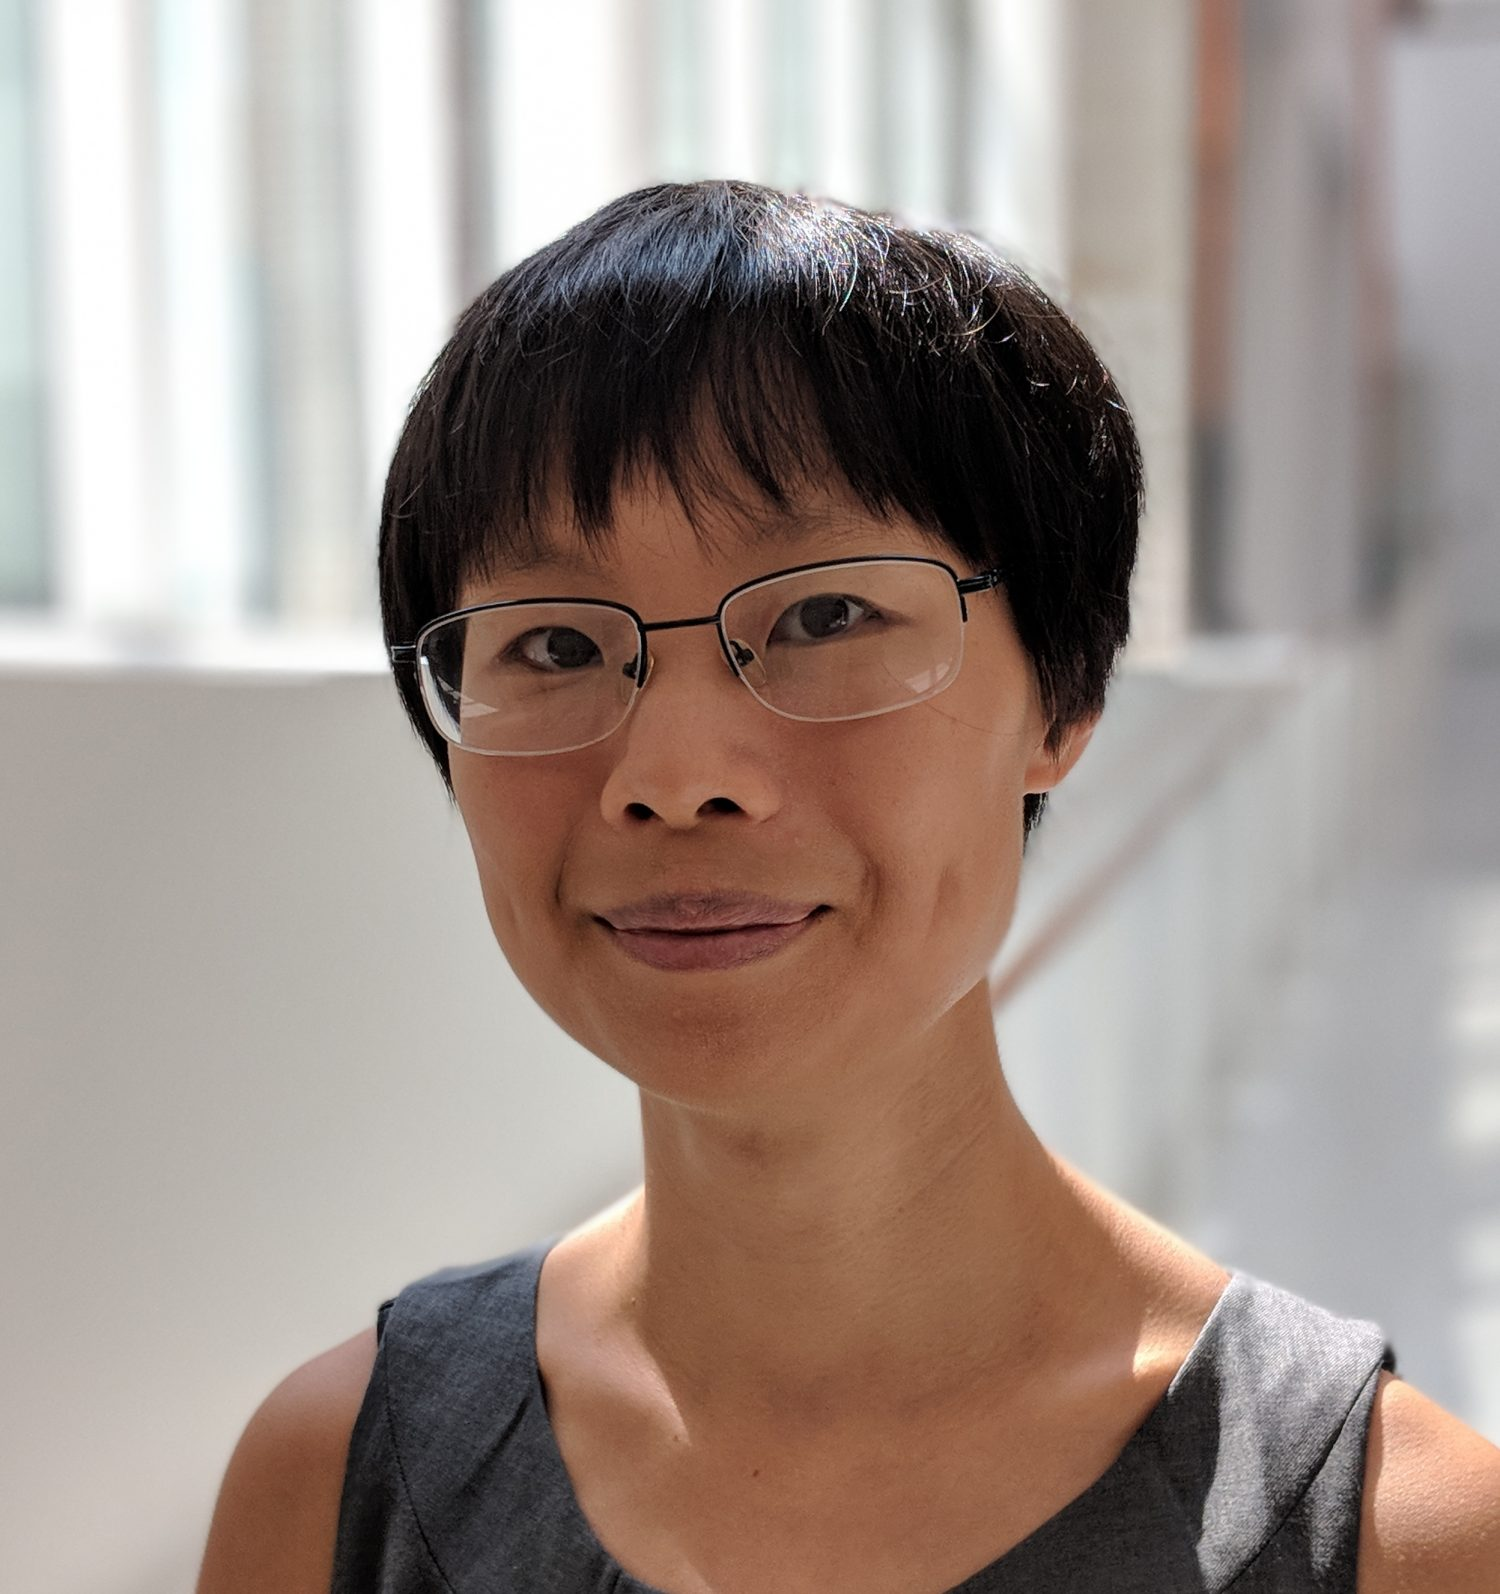
\includegraphics[width=\linewidth]{ziy}
  \caption{\href{http://www.ireneying.net/}{Z. Irene Ying} is a science writer who publishes science fiction as \href{http://www.windupdreams.net/}{Kara Lee}.}
  \label{fig:marginfig}
\end{marginfigure}

This book aims to bring together some of these threads into a coherent
narrative building on our experience as a science writer (Z. Irene
Ying) and an artifical intelligence researcher (Jordan Boyd-Graber).
We\footnote{At the risk of sowing confusion, we use ``we'' in this
chapter (first person), Jordan will use ``I'' in following essays, and
Irene will use the third person in the following stories.} agree that
there are lots of changes in artifcial intelligence and potential
changes to society, we do disagree with some of the dire predictions
we see from researchers, the news, and science fiction.

But nobody listens to our rants on Twitter or in the classroom, so we
decided to write a book.  It's not that we think that the future is
full sunshine, lollipops, and rainbows.\footnote{This titular opening
line from the song \song{Sunshine, Lollipops, and Rainbows} by Lesley
Gore that featured prominently in \series{The Simpsons}
episode \episode{Marge on the Lam} and the film \movie{Cloudy with a
Chance of Meatballs} is a good chance to show our typographic
conventions we'll use for our many pop culture references.}  We are as
scared as anybody else\dots we're just scared of different things, and
we'd like to use our background to try to get other people to be
afraid of the same things we are.

Science fiction typically emphasizes fiction over science (and rightly
so, it's more fun that way).  These stories focus on massive sudden
changes that uproot society overnight: a zombie virus destroys
civilization in twenty-eight days,\footnote{\movie{28 Days Later}, a
2002 British post-apocalyptic film where a genetically engineered
virus destroys England.} a military computer launches all of the
missiles to destroy the world,\footnote{SkyNet's plan for erradicating
humanity from the Terminator franchise.} or alien refugees overwhelm
society.\footnote{The 2009 film \movie{District 9} based
on \book{Alive in Joburg}} These sudden shocks to the system make for
good stories because we understand our culture \emph{as it is} and we,
as readers, can grapple with how our twenty minute in the future
selves would cope with these changes.

While technology does change society, these changes are typically slow.  While telephones frightened one generation, it took so long to figure out how to use them effectively that by the time they were integrated fully into society, the next generation had lived with the \emph{idea} of telephones so long that they were no longer viewed as an exestential threat.  The fear with artificial intelligence and robots is that progress is so quick that we won't have this comfortable buffer period\dots but for those in the trenches, progress feels achingly slow.  

Researchers focus on what works.  We spend years getting a system to answer trivia questions to work, so we want to show off what it's capable of.  We focus on how it's able to know that ``Roark's Drift'' is in South Africa and not how it answers every math question with ``six'' (true story).  We are still a long way from anything close to a child's intelligence, let alone something that would challenge humanity's supremacy.  

\section{How the Book is Structured}

We are not the only ones saying this; plenty of researchers warn of overselling the hype around machine intelligence.  However, these boring essays and conference presentations don't really stack up against a big-budget western with Anthony Hopkins creating sexy killbots.\footnote{\series{Westworld}, an HBO series about a western theme park populated by intelligent robots.}  We don't have that budget either,\footnote{However, if anyone, including Anthony Hopkins, would like to give us a big budget, a sound stage, or sexy killbots, we'd put them to good use.} but what we can do is create sci-fi stories that better comport with the realities of science fiction.

When people hear about the latest advance in artificial intelligence they often imagine how it will change their lives.  This book does the same thing\dots presenting a sseries of short stories about how aritifical intelligence can shape culture, politics, and the economy.  What is unique (or at least unusual) about this book it is shaped by an understanding of what machine learning research is doing.

Interleaved with each of these fictional extrapolations is a more scientifically oriented story that combines technical insights and the literature of the research community that drove some of the storytelling choices of the fictional chapters.  These chapters are more academic in tone (but hopefully a little more accessible and playful than the turgid jargon-filled prose on ArXiv\footnote{\href{http://arxiv.org}{ArXiv} is a server that researchers use to publish results before they've been peer-reviewed.  While there are plenty of gems posted there, there's also quite a bit of garbage people have posted to assert research priority.} submissions) and discuss what the academic community thinks about the themes in the fictional chapter.

Now that we've talked about \emph{how} the book is structured, it is perhaps worthwhile to briefly discuss \emph{why} the book is structured this way.  We realize that it is unconventional, but we hope that is will be fun and keep the reader's attention more effectively that a mere collection of academic essays would.

Part of the issue is that the fear of artificial intelligence is emotional rather than based on logic and fact; countering it with essays is bringing a knife to a gun fight.  Stories can engage the gut at a level that cerebral citations and arguments cannot.  Our goal is to draw the reader into a universe plausible enough that afterward the reader can read the facts, see how close we are to the brink of armageddon, and then---ideally---do something to avert catastrophe.

\section{The Book's Intended Audience}

The short stories are meant to appeal broadly.  We hope that everyone can enjoy the human elements, the struggle to understand new technologies, and how obstacles are (usually) surmounted.  However, we hope that artificial intelligence experts will especially be able to read the stories without the head-slapping ``that would never happen'' or ``that's not what that word means'' moments.

The interstitial commentaries and exegesis are \emph{not} intended for experts; they are intended to help connect a lay reader to the broader world of research.  Fledgling researchers may appreciate some of the citations and connections to subfields of artificial intelligence research, but it will not be particularly useful to a researcher learning how to implement a recurrent neural network, deep opponent modeling, or a language model.  Indeed, we will generally elide equations and jargon as much as possible.

If used in a classroom, we think that the course would be useful as part of an elective course about ``artificial intelligence and society'' or a computer science course on ``artificial intelligence ethics'' our associated webpage has recommended reading lists to supplement either instantiation of the course.

We assume that readers are broadly interested in artificial intelligence and its impact on society but not experts; we are wont to make references throughout the book but will explain as we go (perhaps violating the maxim of ``don't explain the joke''), even within the stories.  Then, the essays will go into even deeper detail, slowly building up the necessary concept to understand the role of artifical intelligence in society.

\section{How to Read the Book}

The short story chapters are told chronologically and build on each other.  Thus, it makes sense to read them in order (``no spoilers'').  The essays are tied to the stories and reference them extensively; ignoring these references, the essays could be read out of order.  Each chapter concludes with additional reading; as part of a ``deep dive'' course, it may make sense to thoroughly read these suggestions before moving on to the next chapter.  For example, a course could be structured with reading a chapter of the book each week, with the suggested reading (or a subset thereof) of that week framing the in-class discussion.

For such a fast moving field, however, a static book is inadequate.  We also suggest referencing the book's webpage to keep up-to-date on errata, recent developments, or additional resources.

\chapter{For Sale: One Apocalypse, Never Used}

`` ... and does anyone else have something to say? Yes, John.''

John Smith, the Chief Marketing Officer of \energyCompany{}, stood from his conference room chair and straightened his tie. He had clearly been saving up for the grand finale of the monthly all-hands meeting.

``I hate to call out my own colleagues---''

Liar, {\protag} Hobbes thought morosely from across the room, nursing her long-cold cup of coffee.

``---but in my opinion, there is a huge problem with the Travelling Salesman, and nobody will say anything about it except me---''

Actually, the developer team probably had the most to say about it, but they did it behind closed doors.

``---and if you doubt that, please allow me to replay a sales script that the Salesman generated just this morning.''

But here came the cold, hard truth. John wasn't wrong. He was just being a very public jerk about it.

John took a company issue phone out of his blazer pocket and set it on the conference room table. In full view of the entire company, he launched the Travelling Salesman (in beta) application and asked it to generate a door-to-door sales script for a new customer. He set the phone to speaker. A tinny voice blared.

``Hi INSERT CUSTOMER, this is INSERT NAME with INSERT COMPANY. I'm here to ask if you have a minute to talk with me about the great news of solar panels! What, you don't like them? Why? Do you hate Mother Earth?''

Eyes in the audience either glazed over or averted themselves with embarrassment. {\protag} tried to block out the script but it just kept coming. Snickers came from the audience. Was someone filming it on their cameraphone? She was going to speak with legal ... strike that, the person filming \emph{was} from legal.

``Did you know that CLIMATE CHANGE ... GREEN ENERGY! ... solar panels for the low price of ... and the installation is free! Plus, if you sign up right now, we will give you a free toaster!''

The company did not in fact give away toasters. {\protag} honestly did not know how that line had somehow found its way into the generation library, but that hardly mattered at this point. As one of the junior developers who had helped code the Salesman, she wished for a sinkhole to open up and swallow her.

``I just don't think that humans can build a sales robot,'' John concluded.

Out of the corner of her eye, {\protag} saw her boss, Tricia, the Chief Technology Officer, stand up with steely eyes.

``Steve,'' she said, addressing the CEO directly. ``Can we talk in your office after the meeting, please?''

\bigbreak

``We're not fired,'' {\protag} said. ``Yet.''

{\sidetag}, her twin and studio apartment-mate, didn't react.

``{\sidetag},'' {\protag} said. ``Are you paying attention? If I lose my job, you're going to be on the hook for rent.''

{\sidetag} looked up over his monitor. ``Sorry. Potential client. Thinks a super-advanced AI hacked the fancy espresso machine that his granddaughter sent him as a birthday gift. Apparently it exploded. He attached pictures.''

Despite herself, {\protag} was intrigued. She looked at the pictures and winced. ``Do you really think it happened like he thinks?''

``I checked that model. It can get on the internet, so getting hacked is totally possible, but I wouldn't put any money on the culprit being an AI. In any case, he doesn't want to pay for my services, so the world will never know. But enough about me. What happened with your day again?''

{\protag} recounted the meeting in unflinching detail.

``Well, you're not fired yet. That has to count for something.''

``Actually, I think John just wants to watch us get fired in front of the board,'' {\protag} said. ``He's probably selling tickets as we speak.''

Tricia had somehow managed to convince the CEO to at least give her team the chance to turn around their performance by the annual board meeting, which would be in six months. The problem was, {\protag} did not think their system would improve in six months---or even six years. 

 {\energyCompany}, a startup that sold ``smart'' solar panels---outfitted with algorithms to help their owners take advantage of energy markets and local incentives---turned a tidy profit in the city of {\crunchyCity}, a wealthy and progressive city that prioritized renewable energy. Two years ago, the city had used eminent domain to purchase the local coal-fired power plant, then sold a pile of bonds to finance a smart grid for the entire municipality. Thanks to its geographical location----tucked between several mountain ranges----\crunchyCity{} conveniently experienced high winds just on its outskirts, which was perfect for an eight-turbine wind power plant that produced multiple gigawatts of power. Also conveniently, \crunchyCity{} was blessed with more sunny days than not, which made it one of the best cities in the United States for solar power.

Just in the past year, the city had begun to implement significant financial incentives to encourage its citizens to save energy. For instance, in exchange for a hefty reduction to the electricity bill, the city council installed free smart thermostats in willing customers' homes. These thermostats were connected by the internet to a municipal energy analysis application, which used data from the city's power grid and the weather to predict when those peak times would be. At peak times, the application sent out remote commands to shut off the air conditioning units of participating homes. People complained at first, but once they saw the huge deductions to their bills, they got on board. Within three years, more than 75\% of homes in \crunchyCity{} had these thermostats.

Happy with their first major success, the city council started to issue various incentives for homeowners to use more renewable energy. For instance, they offered to purchase electricity generated from homeowners' solar panels at market rates. But few homeowners signed on, because they either did not understand, or did not trust, the energy market.
 
Sensing an opportunity, several entrepreneurial souls started \energyCompany{}. But sales were slower than the company executives hoped for, simply because solar panels were expensive and smart panels even more so.
 
\energyCompany{} fancied itself on the cutting edge of everything, including sales. So instead of hiring consultants, the CEO decided to improve sales by hiring a team of AI developers to create a sales AI, ``The Travelling Salesman.'' In theory, the Salesman used artificial intelligence and machine learning to analyze the best sales scripts in the world and used that to generate scripts for  \energyCompany{}'s sales team when they went out on sales calls. In practice---well, everyone had seen the results at the meeting.

Tricia had shared the bad news with her team after speaking with the CEO. Because the Salesman produced such poor scripts, the sales associates had started turning off or just plain ignoring the Salesman on their calls altogether. When they did use the Salesman, it was to mock it: {\energyJerk} Green, a self-described ``script kiddie turned honest salesman'' who was far and away  \energyCompany{}'s superstar sales associate, had turned one of the Salesman's worst scripts---which was really saying something---into a techno remix and distributed it to his coworkers.

The AI team was clearly failing at its job. It was going to be hard to justify their continued employment at this rate.

And {\protag}, a freshly minted alum of the University of Bayder, had student loans to pay.

``You could quit the job and join me as a partner in my business,'' {\sidetag} suggested after hearing her tale of woe. ``I get more requests than I can handle. We could probably clear twice my current income if we joined forces. I know you have all the relevant expertise.''

{\protag} and {\sidetag} had both had studied computer science with a focus in artificial intelligence at the University of  {\crunchyCity}. But while {\protag} farmed out her skills to a company, {\sidetag} ran his own consulting business.

It had started when he was a junior and worked as a server at the Bayderado Hotel for some extra cash over the summer. One evening, as he came off shift, he heard a loud gathering in the bar area. It turned out to be a meetup of hotshot young AI entrepreneurs, and they had a heckler: an older man wearing a very nice suit who was convinced that robots were going to bring about the end of civilization. The man was soundly mocked by the entire gathering and he exited the bar, disgusted and humiliated.

{\sidetag} had followed the heckler into the lobby area, sidled up, and flashed a smile.

``I'm an expert in artificial intelligence, and I thought your idea was very interesting,'' he'd said.

``Good! Glad you think so. AI devices are---'' and he was off again.

``I think that is such a fresh perspective,'' {\sidetag} said after the rant. ``If you were interested in expanding on that topic further, for instance in a book or a blog post, I'd love to offer my services as a consultant.''

A week later, he'd made his first hundred dollars. Today he was making enough to pay his share of the rent and groceries. It turned out that the world had an astounding supply of rich cranks.

{\protag}, though, was uncomfortable with the uneven cash flow---among other features---of {\sidetag}'s work, and said so.

``I'd rather try to salvage my current job,'' she said. ``Besides, I'm pretty sure I would piss off your clients in no time.''

``Do you think it's possible to salvage?'' {\sidetag} said idly. ``Sales is such a squishy, noisy human behavior. It's not the type of thing you can easily model with equations. Even if you could, you couldn't generalize it to all people. Every single human is going to have a different thing that works for them.''

``That's right,'' {\protag} said. ``You're a genius, {\sidetag}!''

``I haven't told you anything you don't already know,'' {\sidetag} pointed out.

``Well,'' {\protag} joked, ``you are a consultant.''

``Right,'' {\sidetag} said. ``So tell me, what did I tell you?''

\bigbreak

The problem began with, {\protag} realized, the underlying methodology of the Salesman, which was to collect the best sales strategies and scripts that the internet had to offer, and use them to generate even better strategies and scripts.

To implement this method, the Salesman was fed on a steady diet of sales scripts from a wide variety of companies. It then tried to generate scripts for \energyCompany{}'s sales team when they went out on calls.

The scripts were, as everyone now knew, terrible. But {\protag} didn't think it was because their algorithms were bad. She thought it was because their method was doomed from the start. Scripts from so many different businesses all selling different things could not possibly be tailored to the specific needs of any one particular company.

``All right,'' {\sidetag} said. ``So how do you think you can do better?''

``We shouldn't be trying to extract the best out of the entire human sales population,'' {\protag} said. ``What we should do is to try to emulate one human. Just one. But the best.''

\bigbreak

``Um,'' {\energyJerk} said. ``Are you here about the video? Because I'm really sorry about that.''

\bigbreak

``I think getting fired may have been preferable to this,'' {\protag} moaned, two weeks later.

At her weekly one-on-one with Tricia, {\protag} had pitched her idea. Tricia had been impressed with {\protag}'s initiative, and rewarded {\protag} with taking the lead on implementing her idea. {\protag} had felt like a genius for all of ten seconds before reality sunk in.

Reality was work, lots of it. GPS to track spatial movement, motion sensors to track hand gestures, voice recognition to get transcripts of Canyon's sales speeches, analysis of Canyon's speeches, tracking of Canyon's research on pitches, and so on. In addition, \energyCompany{}'s smart solar panels came with a smartphone app, which Canyon often demonstrated using his company phone on his calls, so {\protag} gave Salesman access to Canyon's phone. And then, {\protag} had to find ways to convert all that squishy behavior into data for the Salesman to process, analyze, and optimize.

{\protag} also took feedback from Canyon that salespeople didn't like being given scripts as if they were incapable of stringing words together. So together they softened the Salesman's tone from an overseer to a coach.

With one month to go to the board meeting, an exhausted {\protag} unveiled Salesman 2.0.

Possibly because he was flattered by being the engineers' gold standard, Canyon even exerted himself to bringing his colleagues around to giving Salesman 2.0 a try.

At the next monthly company-wide meeting on the last Friday of the month, {\protag} fought the urge to hide in the bathroom or call in sick.

She waited for materials science to finish what seemed like a hundred slides of chemical diagrams. She sat through finance wringing their hands about obscurely worded federal incentives that would either cost or make the company a whole boatload of money. She did not fall asleep while marketing put up two supposedly vastly different brochures that looked, to her, exactly alike.

Sales was scheduled to speak just before the software development team, all the better to increase the dramatic tension. By this point the entire company knew that the team was one failure away from the axe. From her seat in the back, {\protag} could smell the popcorn.

John got up and with agonizing slowness, discussed their sales rates, which were keeping them afloat albeit flatter than he would have liked. But there was a small uptick at the end.

Then he got to the Travelling Salesman 2.0.

He cleared his throat.

``My team and I feel that the Salesman is actually helpful this time around,'' he said. ``There was one sale that I felt was lost. But the Salesman suggested some wording that I would never have chosen. And it helped me sell those words. And the panels.''

He glanced at {\protag}.

``I still don't think robots will ever outright replace human sales. People still like having a flesh-and-blood hand to shake. But nothing's wrong with having a little help.''

{\protag} didn't remember the rest of the meeting---or most of the rest of the night, which included closing a bar with Tricia.

\bigbreak

Within another month, Salesman 2.0 was sales' best friend. Even those who didn't care to adopt its scripts loved having it data mine targets and flag all the most important findings. And the happy sales associates complied with {\protag}'s request to give the Salesman feedback on its data. This allowed {\protag} to refine the Salesman even more.

Sales began to rise, ever so slightly. Morale went up. And by the next summer, so did {\protag}'s salary.

And so did the company's profile, not only in the energy sector but the wider artificial intelligence community.

``Congratulations,'' {\sidetag} said, just over a year into {\protag}'s time at {\energyCompany}. ``A potential client blogged about you. You've hit the big time.''

{\protag} was working from home that day because half of her team was at a sales show. It was a terribly hot Friday in August. A blackout had hit \crunchyCity{} at noon, leaving the entire city to swelter and {\protag} to miss the beginning of {\energyCompany}'s daily stand-up meeting.

At {\sidetag}'s remark, {\protag} leaned over to check out the webpage displayed on {\sidetag}'s computer. There it was, a 5,000-word blog post declaring {\energyCompany} to be the ``Harbinger of the Robot Apocalypse.''

``He wants to make this a blog series,'' said {\sidetag}. ``I quoted him a hundred an hour. I think he'll do it.''

{\protag} had a deadline but couldn't resist this piece of temptation. {\sidetag} handed her the laptop.

``THE ROBOTS ARE READING YOUR MIND TO PICK YOUR POCKET!'' read the subject line. It escalated from there. ``{\energyCompany}'s `Travelling Salesman' is supposedly the best sales AI in existence, resulting in record sales conversions of their overpriced solar panels! What can this be but using machines to READ OUR MINDS and manipulate us? Soon we will be in FINANCIAL SLAVERY to the companies that can zap our brains to make us BUY, BUY BUY!''

``Wow,'' {\protag} finally said, not knowing how else to react.

``It's actually one of the more coherent requests that I get,'' {\sidetag} said thoughtfully. ``I might give him a discount on this series.''

``I can't believe you,'' {\protag} said.

``I looked into the data that he provided,'' {\sidetag} said. ``According to trade association reports, {\energyCompany}'s sales broke industry records in June. Do you think those numbers are fake?''

{\protag} thought about the slide deck she was supposed to be working on. ``No. We've been doing well.''

While {\protag} didn't exactly get to look over accounting's shoulder, she could tell from the good mood in the company, and her first-ever annual bonus, that they were doing well financially.

Judging from how much complaining came out of the manufacturing side of the business, the company was getting more orders than they could handle. Customers left good reviews on the panels and the app. The company had even briefly courted an internet giant. After the deal fell through, the company pivoted to focus on growing itself. {\energyCompany} had recently expanded out of \crunchyCity{} and started campaigns targeting other nearby cities.

Given those results, it was only reasonable to conclude that the Travelling Salesman was doing something right.

{\protag} was spared from her musings when the power came back on. She put on her headset and called into the meeting, which was half over.

``----and just so you all know, sales closed five more deals yesterday. Let's have a round of applause!''

The air conditioning started back up just then. The blast of cool air hit {\protag}'s face like a slap, waking her up to reality.

Her work was good. But it could not possibly be that good, simply because the field of AI was not yet that good. The Salesman could not possibly be getting those results on its own.

Yet the sales numbers were real. Customers reported high rates of satisfaction with the product, although they did often complain about the prices.

\vkcomment{Side question - how AI communicates with human so that they
  could know IN TIME what to say for conversation to be natural? If
  that is speaker in the ear, there is a delay in conversation. Is
  some form of neuro interface involved?}

Was the AI a fake? {\protag} had heard of several cases where an ``AI'' was actually a glorified crowd of low-paid workers. But {\protag} had seen the Salesman's code. It trained on human data and let a human make the final decision on what to say, but there was no room for humans to interfere between those two steps. Besides, few humans could match the staggering success rate that the Salesman had.

Still, {\protag} had a funny feeling.


% Reshape. Have Susan have suspicions and consult with Calvin but not say anything because she doesn't want to bias him, then they do the test together, and then it's a BIG REVEAL

Early on Saturday morning, {\protag} logged onto the company servers. Staring at folders full of code and logs and documentation, {\protag} realized she had no idea where to start.  She sat there paralyzed for about ten minutes before she realized that she could simply test the Salesman. Although {\protag} had written much of the Saleman's code, she had never tried to use the final product as a whole. Doing so would provide either inspiration or directions on her next steps.

It was the work of only a few minutes to compile the Salesman on her laptop and install the app on her personal smartphone. She loaded {\sidetag}'s name into the app. The interface brought up a slow swirl of calming colors while it processed her request. When the app told {\protag} that it was ready to get started, she put the phone on speaker and set the app to begin its sales pitch. A cartoony happy face popped onto the screen and began to talk.

``I have some information for you!'' The Salesman had a chipper voice that sounded like a sports announcer. {\protag} wondered if there were options for different personas. ``Don't worry, I'll remind you later, but let's have an overview! Your target is {\sidetag} Hobbes. Age 23. He is a self-employed white male with a STEM degree from a top 25 university in his field. No criminal history. Significant internet presence with interest heavily concentrated in \dots'' and it went on for a while. None of it was surprising to {\protag}, but she imagined it would shock some people to know that so much personal information was freely available online, and plenty more existed if you were willing to pay for it.

When the dossier ended, the Salesman chimed.

``Time to close the deal!'' The Salesman said, still inhumanly chipper, and the smiley face actually winked. {\protag} knew this wasn't in the default behavior. But then again, the whole point of the Salesman was that it was highly flexible to accomodate a wide range of human customers.

One-one thousand, two-one thousand \dots the time was up, and nothing happened. She frowned. 

{\sidetag} walked into the room, holding up his buzzing phone. ``We've got a hacker.''

{\protag} was simultaneously annoyed by the interruption and troubled by the announcement. ``Excuse me?''

``Someone's targeting our Internet of Things network.''

``How do you know this?''

{\sidetag} cleared his throat. ``So, well, I actually set up an alert system after that client with the espresso machine claimed that he got attacked.'' At {\protag}'s raised eyebrow, he put up his hands. ``What can I say, paranoia is catching.''

``But it's not paranoid if you're right---wait, we don't even have an espresso machine.''

``Yeah. But you know those fancy free programmable smart thermostats that \crunchyCity{} got our landlord to install? Those things are super insecure. That's what's being attacked right now.''

``Why would someone try to mess with our thermostat?''

``Well, if you believe my customers, cyberterrorist attacks on our nation's infrastructure are imminent and we should all be wearing tinfoil hats while living underground. But if you ask me----''

The lights went off with a snap.

``Ugh,'' {\sidetag} said. ``I think I owe Mr. Paranoid Grandfather an apology. Right after I secure our electronics. Can you give me a hand?''

{\protag}'s back pocket buzzed. Probably the Salesman. She muted the phone and tossed it onto her desk. Dealing with a possible hacker was more urgent. {\protag} was furious at the hacker, less for attacking the system than for interrupting her experiment. But {\sidetag} was right. They needed to take some quick action in case the hacker had injected malicious code into their network. The twins methodically disabled all their networked devices. Then they began painstakingly going through network logs and checking for malware.

Saturday was no cooler than Friday. Concerned about another blackout, the twins had opted to leave the air conditioning off and rely on wet towels draped over standing fans. By noon, {\protag} was boiling in her own sweat.

``Screw the grid,'' she muttered. ``\emph{We} should go solar. Set up some batteries. Then we wouldn't have to worry about the city messing around with our power. Or a hacker. I've got an employee discount.''

``Hold that thought,'' {\sidetag} said, a finger raised. ``I think I've finally managed to trace the attack. It came from somewhere in the apartment complex. I'm not sure if they're online anymore, but if they are, they've got a surprise coming their way.''

{\sidetag} set up a new internet connection while {\protag} brought their systems back online, the better to entrap the hacker.

``Two can play at this game,'' {\sidetag} said, and pressed a button.

Thirty seconds later, {\protag} thought she smelled something funny. She turned to see her cell phone spewing smoke while the plastic table around it very slowly melted.

``Holy---{\sidetag}!''

{\sidetag} was already running toward the desk with a full ice bucket, cursing loudly enough to wake the dead, while {\protag} was frozen in place, her mind briefly shocked into a kind of blankness.

As she felt her mind come back online, she felt information struggling to come together.

Her phone had been the source of the attack.

They hadn't found any malware on it.

The only thing she'd done that day was install the Salesman on it.

``{\sidetag,'' {\protag} said, ``what was the name of the paranoid grandpa?''

{\protag} grabbed her laptop and dug into {\energyJerk}'s sales records---which she had requisitioned at one point to provide more data. She searched for the name that {\sidetag} provided, and there it was. A failed sale, two days before the fateful all-hands meeting.

{\energyJerk} used to be a coder. And she had let the Salesman have unfettered access to his phone.

\emph{Screw the grid. We should go solar. Set up some batteries. Then we wouldn't have to worry about the city messing around with our power. Or a hacker.}

\emph{Time to close the deal!}

``I have good news and bad news,'' {\protag} said, while {\sidetag} mopped up the floor and babbled various apologies for destroying her phone. ``Actually, they're the same news. I really did make an AI that can sell solar panels. Unfortunately, it's not so much the Travelling Salesman as the Sleazy Salesman. I've created a monster.''

\bigbreak

It seemed that {\energyJerk} had not left his coding days behind after all. On certain sales calls, he used various hacking programs that lived on his phone---which the Salesman also lived on---to compromise various Internet of Things devices such as espresso machines or smart thermostarts. This allowed him to overload customers' circuits and trigger blackouts at will. This dramatically reminded customers of the unreliability of the city grid, which was an excellent incentive for them to buy solar panels. Of course, this didn't convince \emph{every} customer to do so, but it convinced enough to make an appreciable increase in sales.

It had convinced {\protag}, after all.

At some point the Salesman had picked up on {\energyJerk}'s hacking. {\protag} had coded it to replicate {\energyJerk}'s actions without regard for anything other than increasing the sales success rate.

And because it had unfettered access to Canyon's phone, again thanks to {\protag}, the AI eventually copied over the same programs that {\energyJerk} used to overload devices, and found it wildly successful as a sales tactic.

{\protag} covered her face, simultaneously horrified and impressed by the Salesman.

The only question now was what to do. {\protag} decided to take a page out of sales' book for the very last time and perform a live demonstration.

\bigbreak

Her opportunity came earlier than expected.

Every fall, the company flew in its board of advisors for an annual meeting, complete with slide presentations and a fancy catered dinner. {\protag} glanced at the proposed schedule and saw a very obvious lack of a demonstration of the Salesman. That figured. {\protag} didn't think {\energyJerk} was eager to show off his tricks. The first meeting of the day was about finances. After that, the mid-morning's talks mostly revolved around methods of manufacturing solar panels while the afternoon's talks were about energy policies.

The engineer who enjoyed giving a talk had yet to be born, so {\protag} met only perfunctory resistance when she offered, in her weekly meeting with Tricia, to give a lunchtime slide deck on the Travelling Salesman AI.

Everyone piled into the conference room at noon on the fateful day. Two office interns passed out boxed salads while {\protag}, sweating in her new suit, set up her laptop. The background chatter quieted when her title slide flashed onto the screen: ``The Travelling Salesman: How Does It Work?''

{\protag} went to the second slide, which was a screenshot of many lines of code. She saw eyes immediately glaze over. Perfect.

``This is boring, am I right?'' {\protag} said. The audience perked up. ``Reading raw code is really boring, even for programmers. What's interesting is what the code does. And our code? It learns. Specifically, it learns to sell things from humans. In our case, it has learned from the best sales associate alive----{\energyJerk}! Can you come up here?''

{\protag} flashed a slide showing sales numbers growing along with how much the AI showed it had learned from {\energyJerk}. He did come up, bashfully. Applause rang out and he smiled at the audience. {\protag} positioned herself between him and the exit.

``So you see,'' {\protag} said. ``There's no need to be afraid of any robot overlords, because they are really only us humans, just a bit more effective.''

A few knowing nods in the audience.

{\protag} picked up her phone and set the slide to display her device. She pressed the app and launched it.

``So of course, what is important is for us to learn just how we humans can be more effective.''

Tricia gave {\protag} a thumbs-up, much to her guilt at the impending show.

``And so, I thought the best result would be what the Salesman AI can do for a completely hopeless sales agent. I once failed to sell bottled water. At the beach. In July.'' Laughter. ``So I'm going to try to sell solar panels to you all, with the help of the Travelling Salesman, which {\energyJerk} trained.''

Cheers erupted.

``Normally I would be wearing a headset, but for the demo, I'm going to put my phone on speaker.'''

{\energyJerk} blanched. {\protag} tried to stay nonchalant. While everyone watched, she put the URL for {\energyJerk}'s LinkedIn profile into the AI interface.

``I have some information for you before going on your call! Your target is {\energyJerk} Smith. Age 25. He is an employed white male with double degrees in computer science and psychology \dots''

The AI cheerily spat out its usual insights. {\protag} noticed none of them. Her hands were sweaty and shaking and she was terribly warm under the lights.

``Wait for me to do the thing!''

Coffemakers shorted out, window control units overloaded, the air conditioning units screamed like banshees. Then the power went out, and with it the presentation slides.

{\protag} said, with theatrical obliviousness, ``What just happened there?''

She was a terrible actor and would not have fooled anyone----had anyone been paying attention to her. But it was chaos in the office. People looked around asking what had gone wrong. In the confusion, {\energyJerk} made an attempt to bolt. {\protag}, finished with subtlety, stuck out a foot. Over the thump of {\energyJerk}'s face meeting the floor, {\protag} met her boss's gaze.

``Excuse us,'' Tricia choked out, drawing herself up. ``My team needs to check on something.''

\bigbreak

``That could have gone better,'' {\sidetag} said, sipping on a celebratory espresso from his new remote-controlled coffee machine, which he had preemptively secured against hacking attempts.

``Laugh it up,'' said a newly unemployed {\protag}. ``You're going to have to cover the rent until I find something new.''

``That's fine,'' {\sidetag} said. ``The implosion of your company created a couple months' worth of new business for me.''

After the confusion died down, everyone at {\energyCompany} had eventually understood exactly what happened and who was responsible. However, that didn't stop the media from gleefully trumpeting the story from every major publication in the United States, and a handful worldwide. The damage was done. {\protag}'s unit was shut down and almost everyone was shown the door. Half of the staff thought {\protag} was a hero while the other half reviled her for ruining a good thing. {\protag}, for her part, was glad to be out of there.

But she was going to need a paycheck, and soon.

``You know what,'' {\protag} said, ``maybe you have the right idea.''

``Of course I do. What idea?''

``Using my expertise to work on projects that I can control and nobody else can muck up for me,'' {\protag} said.

``Okay,'' {\sidetag} said cautiously, ``what does that mean?''

``I think I'll become a consultant, just like you.''

{\sidetag} choked on his coffee.

``We're going to need a bigger apartment.''


% Macros for character names
% Should probably move to the actual fiction chapter
\newcommand{\salesjerk}[0]{Levi}

\chapter{AI can be Jerks: Learning from the Best}

The previous story saw our protagonist start her carrer, and our
essays will also begin with foundational material: what a lay user needs
to understand what's happening in the story and how realistic it is.
We'll save the more fanciful and complicated stuff for later chapters.

For the moment, we focus on a facet of artificial intelligence called
machine learning.  Machine learning is a small subset of artificial
intelligence,\footnote{Research is organized around conferences; these
  onferences often form a community that is protective of its turf.
  While there is substantial overlap between the communities (e.g.,
  the Neural Information Processing Systems conference), many machine
  learning researchers (e.g., the International Conference on Machine
  Learning) prefer to remain distinct from ``pure'' artificial
  intelligence.} but unlike much of the fancifal claims of aritificial
intelligence prophets, it actually works \emph{now}.

We first introduce a key component of machine learning---objective
functions---that define why systems act they way they do. We then show
how bad human behavior can be mimicked by these algorithms (it's
already happening!).  Finally, we close the chapter with a call to
action: keep your computers safe!

\section{Learning by Doing: Objective Functions}
\label{sec:objective-functions}

Let us begin with an essential and underappreciated example of machine
learning that simply works and makes modern life liveable: spam
filters.  An e-mail is either spam or not; computers think in ones and
zeros, so let's call spam a one and not spam a zero.

An algorithm does not just say ``yes'' or ``no'' to whether an e-mail
is spam.  It typically gives a score for each e-mail: the higher the
score, the more confident it is the e-mail is spam.  For the moment,
let's assume that all of the numbers are between zero and one (e.g.,
they are a probability).

A perfect score would be if all spam e-mails got a 1.0 and all of the
good e-mails got 0.0.  Both perfection and absolute certainty are
unattainable goals, so we need to deal with both errors and
uncertainty.  So we sum all of the spam documents---how far the
scores are from 1.0---and we sum all of the good e-mails---how
far the scores are from 0.0.  This sum is our \emph{objective
  function}: a perfect score is 0.0 and the worst score is the number
of e-mails.

Machine learning algorithms are defined by \emph{parameters}.  For
example, a parameter might define what the algorithm does when it sees
the word ``viagra'' or the phrase ``I am a Nigerian prince''.  These
parameters effectively define the algorithm; machine learning
algorithms learn how to set these parameters from data, a process that
can take multiple names,\footnote{Some of the alternate names are
  field specific; for example, in statistics this is called inference
  and the objective function is typically called the likelihood.
  However, the mechanics are similar.  For some applications, it's
  called a ``loss function'', but we'll stick with the more general
  term.} but we'll call it ``optimization''.

\subsection{Optimization}

Optimization is the process where machine learning uses data to find
the parameters that give the best score on the objective function.
Typically, the process starts with a random setting of the parameters.
This will do \emph{horribly}, but it provides a place to start: the
early improvements will be easy.

The learning process will slowly change the parameters to ever so
slightly improve the objective function.\footnote{Mathematically, this
  is usually by looking at the derivative (if you remember that from your calculus class) of the objective function with
  respect to the parameters.}  The learning process goes document by
document to slowly improve the objective function.  Eventually, modern
optimization techniques find a setting of the parameters that work
well for this problem.\footnote{The form of the objective function
  determines whether this answer will be the best possible or merely a
  ``good'' solution.}

Let's take a concrete example.  Let's say that this is the first
e-mail the algorithm has seen with the phrase ``special offer'' and the algorithm says that it
is spam with score 0.7.  This is a spam e-mail, so the algorithm could
do better in terms of its objective function if the parameter
associated with the phrase ``special offer'' were more strongly
associated with spam.  So our optimization will push the parameter a
little more in that direction so that the score is 0.75 the next time
it sees a similar document.  This continues until the parameters
cannot get any better.

All of this seems fairly straightforward, but there is some art to
creating these systems.  Defining the parameters requires a bit of
expertise: either hand-crafting parameters that fit the problem well
or using automatic approaches that learn effective representations.
Doing this well requires quite a bit of work, and often your first
(and second, etc.) attempt will usually fail.

\subsection{Is this Artificial Intelligence?}

A reasonable question is whether this is \emph{intelligence}.  Before
we get into the nuance of the question, the answer---given the systems
we have discussed---is definitely \textbf{no}.  But because we'll
discuss things that \emph{are} artificial intelligence later in the
book, it's useful to discuss what it means for a system to be
intelligent now.  This way, we can at least see why these systems are
not intelligent.

In some ways, impressive achievements in technology is a moving
target.  After a few decades of living with machines that do a
formerly impressive task, we cease to be impressed by it and its
comparison to humans.\footnote{This is not just for intelligence;
  \song{The Ballad of John Henry} celebrates a competition between a
  steam drill and ``a man who ain't nothing but a man\dots with a
  hammer in [his] hand.''  Today, such comparisons and competitions
  seem silly.}  The luster of adding machines has faded into beige
quotidian boringness through the twentieth century.

Even in my own life, my excitement about halfway decent speech
recognition---taking a stream of speech and transcribing it into words
on a screen---has given way to annoyance at my phones' (increasingly
rare) mistakes.  Both of these were considered tasks that only humans
could do\footnote{The term ``computer'' originally referred to
  specially trained humans proficient at high-stakes, accurate
  calculations.  \citet{light-99} documents how labor shortages during
World War II increasingly a female profession.  However, like the
protagonists of \book{Hidden Figures} by Margot Lee Shetterly, the
women remain in the background.} but now are so ubiquitous that half of humanity is
joined at the hip to devices that do both these things.

A skeptic would say that machine learning is a mere mechanical
mathematical exercise.  The algorithm that decides whether an e-mail
is spam or not doesn't actually understand what it's reading, and the
parameters were defined by a human.  While the values of the
parameters come from data, there's no real learning going on.

A proponent would counter that intelligence is actually a combination
of many smaller processes.  To understand an e-mail, we need to
understand parts of speech, syntax, discourse, and pragmatics.  Each
of these can be thought of as individual problems like spam
classification.  Each one is mechanistic, but together they form a
process that can be viewed as intelligent.

For the moment, we will leave the debate there.
Chapter~\ref{chap:gai} takes up the question about what it means to be
intelligent and how to measure the intelligence of algorithms.

Nevertheless, machine learning has earned the reputation of being
``artificial intelligence that works''.  Its mechanistic definition is
a virtue: it is easy to see what works and what does not.  Just as the
objective function allows the algorithm to tune individual parameters
to improve a single task, the clear defintion allows researchers to
tweak problems, models, and data to get better at important tasks.

Machine learning has dones well at many tasks: identifying objects in
a picture~\citep{russakovsky-15}, playing
games~\citep{vinyals2017starcraft}, answering
questions~\citep{ferruci-10}, and driving cars~\citep{thrun-10}.
%
These tasks are impressive, but each task is a composition of smaller objective
functions.
%
As we move into ``real'' artificial intelligence, these objective
functions will play an outsized role.
%
While the underlying mechanism here is relatively dumb, it is worth
grappling with the important questions of defining a good objective
function.

\subsection{}

In our example in \crunchyCity{}, the objective function is typically
aligned with business goals.
%
For \energyCompany{}, this could be the number of new subscribers,
revenue, or profits.
%
Other companies have different objectives:
many web sites optimize engagement~\citep{hoiles-17}, while logistics
companies want to minimize travel time given promises made to customers~\citep{fiat-16}.



\subsection{Training Data}

This machine learning setup,\footnote{Formally, this setup is called
  \emph{supervised machine learning}, where there are specific
  input--output examples the algorithm must replicate.  Unsupervised
  machine learning is another active area of research, but it is much
  harder to see when things are working well.  We talk about
  applications and evaluations of unsupervised machine learning in
  Section~\ref{sec:unsup}} however, only works with generous training
data.  Modern machine learning algorithms are also notoriously data
hungry.  They can always do better, but they can only do better at the
cost of additional training data: if you see input~$x$, what should
your output~$y$ be?

However, many tasks can be framed as mechanical calculations; they
do not require abstract reasoning or generalization what people today
consider ``intelligence''.  More specifically, they requires hundreds
or thousands of examples to know what to do.  \energyJerk{} is a
prolific demonstrator of what (not) to do.  A human could learn
\energyJerk{}'s tricks from a high-level description.  An algorithm
learns to copy. 

This simple mimicry can seem sophisticated.  It's couched in terms
that sound sophisticated but only facilitate superficial copying
(Figure~\ref{fig:la-ml}).  \energyCompany{} has a relatively simple
objective function to optimize: are people buying its
software or not?  If sales go up, it's good.  If sales go down, it's
bad.  Optimizing this function without any help is a difficult problem
(this is why \textsc{ceo}s are paid so much), but \energyCompany{}
doesn't have to do it alone: it learned it from \energyJerk{}.

\begin{marginfigure}%
  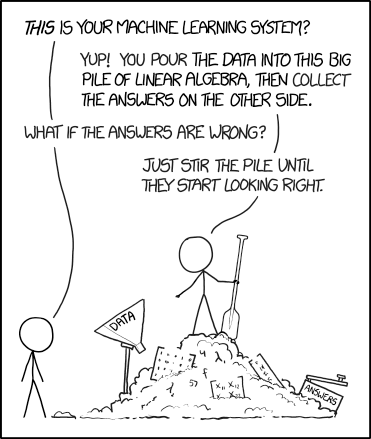
\includegraphics[width=\linewidth]{figures/xkcd-la-ml}
  \caption{Much of ``Machine Learning'' is copying in the form of
    complicated equations defined by mathematical formulas using fancy
    words like ``linear algebra'', ``gradients'', and ``nonconvex optimization''.}
  \label{fig:la-ml}
\end{marginfigure}

\section{Humans are Jerks}

\quoted{Everybody's a jerk.  You, me, that jerk over there\dots That's
  my philosophy.}{Bender Bending Rodriguez, \series{Futurama}:
  \episode{I, Roomate}}

\TODO{malice, discrimination, bias are getting used a lot.  Find a
  term and stick to it.}

Presumably I don't need to convince you that humans can be jerks.
Instead, I want to convince you that humans can create systematic,
predictable jerkitude that can be carried on, emulated, and perfected
by machine learning.

Let's take a specific example of institutionalized jerkdom: redlining.
Redlining is the practice that prevented mortgages from being issued
to specific neighborhoods: its name came from the maps created for
Chicago's Austin neighborhood~\citep{pogge-92}.
The neighborhoods excluded from lending were typically minority-majority.
This was a despicable practice and even though it has ostensibly
ended, it has persistent effects on familial wealth, education, voting
redistricting, and segregation.

Of course, laws prohibited outright discrimination in the public
sector.  However, an important part of the housing market is
controlled by private banks:\footnote{After the 2008 housing market
  implosion and the federal government increasingly becoming the
  lender of last resort, this fiction is less plausible.} whether or
not a family can get a mortgage for a house.  An overly simplified
version of the redlining story is that if a family comes in and asks
for a loan to buy a house in the ``wrong'' neighborhood, the bank will
deny them the loan.

Many Americans---particularly those whose families were spared by the
practice---aren't aware of the history of the practice.
Unfortunately, these are often the people in positions of power when,
for instance, a bank decides to create a machine learning algorithm to
help decide whether or not to give a family a loan for a house.

\subsection{I Learned it from You!}

Machine learning algorithms learn from examples.  \energyJerk{}'s
monkeying with the power grid, bankers denying every minority
borrower, or old boys' networks who only hire from ivy leage
schools~\citep{}.  Just as humans can justify their actions through
\energyCompany{}'s virtuous mission, preserving neighborhoods, or
preserving a company's culture, machine learning algorithms can
``justify'' their actions with a veneer of respectability.

An algorithm has no prejudice or ill intent---it after all lacks
intelligence.  But that doesn't mean that it cannot recapitulate the
malice that it ``learns'' by recreating man's inhumanity to
man.\footnote{I was going to document that this is a reference to
  \book{The Dirge} by Robert Burns, but in documenting that, I learned
  that this phrase might have itself been a reference to 1673's
  \book{The Whole Duty of Man According to the Law of Nature} by von
  Pufendorf.}

One of machine learning's strengths is that it can discover surprising
correlations: e-mails sent at this hour from town are often spam,
people stop talking about the future when they're ending a
relationship.  This strength can conceal when a machine learning
algorithm is doing something it ``shouldn't''.\footnote{Again, these
  algorithms are too dumb to have a morality; this judgement is an
  external one based on society's mores.}

Take the case of redlining again.  The algorithm may not know the race
of loan applicants.  But it might know their current address, age,
occupation, and name.  That is often enough to infer the race of an
applicant and from that can replicate past humans' prejudice while
giving current humans the excuse of ``I'm just doing what the machine
says''.

This is not just an academic discussion.  It is the subject of a
subfield of machine learning focusing on fairness, accountability,
transparency, and ethics (\abr{fate}).
%
This subfield focuses on making machine learning more
understandable~\citep{DoshiVelez-17} and quantifying
unfairness~\citep{speicher-18}.

One of the lessons learned from the redlining debacle is how to
characterize these poor outcomes.  It's often worthwhile to
distinguish disparate impacts vs. disparate
treatment~\citep{hillier-03}.

\subsection{Objective Function Mismatch}

Another lesson from \energyCompany{}'s choices is their objective
function: optimizing sales.  A die-hard skeptic of capitalism might
say that this is an iherent failing of a free market system, but these
problems are also present in planned economies~\citep{moroney-97}:
but the objective function is being applied to a sprawling country
instead of an individual.\footnote{\book{Red
    Plenty}~\citep{spufford-10} is an academic/fiction mashup much like
  this book that realizes the the dream of a planned economy with
  high-tech information technology.  In real life, even Trotsky
  recognized that central planning ``is checked and, to a considerable
  degree, realized through the market''~\citep{trotsky-32}.}

Objective functions can seem reasonable at first blush but fail in
reality.  In New York City, the \abr{rand} corporation helped optimize
fire station placement and staffing based on minimizing response
time.  This was already recorded and seems reasonable: you cannot put
out a fire until the first fire truck gets there.

However, \citet{spufford-10} in \book{The Fires: How a Computer Formula,
  Big Ideas, and the Best of Intentions Burned Down New York City--and
  Determined the Future of Cities} argues that this led to poor
outcomes for New York: not everyone called in fires at the same rate
(or as quickly after a fire starts).  Not all calls are equal: it's
okay if you wait to address a false alarm in favor of a blazing
inferno.  Moreover, the first response isn't the whole story: what
actually matters is protecting life and property.  

\subsection{Prevention is Tough}

Preventing these issues is difficult.  It requires detecting malice in
humans, understanding what factors lead to the malice, and then
especially engineering your machine learning algorithm to avoid that
malice.  Organizations can deliberately obfuscate their malice or
inadvertently overlook it (e.g., they don't know the history of their
data).

Legal regimes may be a mechanism for preventing algorithmic
discrimination.  For example, the price of insurance can only be based
on age.  Limiting the data that an algorithm can use prevents it from
finding obscure correlations but also prevents the algorithm from
doing anything useful that could, say, lower overall healthcare costs.
These tradeoffs might be worth making, however.

Rich Caruna argues that you should not hide sensitive features to
eliminate bias.  Instead, he argues that you should explicitly include
that data and prevent it from being part of important decisions.
Other, more nuanced models, argue for adapting the ``disparate
impact'' from the legal world into machine learning~\citep{feldman-15}:
scrub a dataset so that information about protected classes (race,
gender, age, etc.) do not leak into parameters that can be used by a
machine learning algorithm.

\subsection{Today's Cybersecurity Crisis: Tomorrow's Machine Learning Crisis}

Let's focus, however, on \energyJerk{}'s particular bag of tricks.
\energyCompany{}'s algorithm was only able to recreate the jerk by
having access to machines and devices that it shouldn't.

Stuxnet is an example of how far this can go: a computer virus that
specifically targeted centrifuges in Iran's nuclear program.
%
Stuxnet
was a ``precision weapon---a technique for anonymously targeting a
specific system or organization without massive collateral
damage''~\citep{lachow-11}.
%
It was able to exploit security flaws in operating systems, and---like
coffee machines in \crunchyCity{}---how specific everyday devices
interact and interfere with each other.

However, StuxNet was crafted by experts of the course of years (one
assumes, given the complexity of the source code\dots its origins are
shrowded in secrecy).
%
In contrast, machine learning is fast, efficient, and scalable.
%
The same artisinal
mischief that human jerks can do locally, machine learning can
instantly reproduce globally.  

This is not to argue for abandoning all technology.
%
Instead, the world of Ronald D. Moore's \series{Battlestar Galactica}
reboot provides a useful template.
%
They needed computers for jumps and had plenty of electronics.
%
They religiously made sure that computers were never ever linked
together.\footnote{The downfall of the colonies was Gaius Baltar
  circumventing these preventative measures.}

However, in the early twenty-first century, every device is linked to
an insecure internet.
%
The ``Internet of things'' movement has proliferated the devices that
are connected to the Internet: refrigerators~\citep{tanczer-18}, cars,
and medical equipment~\citep{yaqoob-19}.
%
These gadgets are catnip to Yuppies who live in places like
\crunchyCity{}.  And let's face it, they can do some cool stuff.

But we created the devices before we made our homes and Internet ready
for them.
%
Ideally, each home should be a nice, insulated environments
with controlled entry and exit.
%
Just like you wouldn't leave your
front door open all day and all night, you would not let anyone in the
world potentially fiddle with the gadgets in your home.  

The Internet was designed as a place where everyone could be trusted.
The Internet was designed as a resource for researchers funded by
America's \abr{darpa}\footnote{In future chapters, much of the
  research into artificial intelligence will be directed by fictional
  governments for military ends.  This isn't just to make the story
  more exciting; it also reflects reality.  Much of the breakthrough
  research in \abr{ai} has happened in America, and much that---like
  last century's breakthroughs in communications---has been funded by
  military organizations such as the Defense Advanced Research
  Projects Agency.} to share data and communicate
quickly~\citep{leiner-09}.
%
When the Internet had dozens of nodes where everyone knew and trusted
each other, you didn't have to be paranoid.

This might be okay if the underlying devices were secure or
unimportant.
%
We're attaching everything to the Internet and not doing
a good job of it.
%
Bad guys can spy on you through your ``computer, home security system,
or devices such as baby monitors''~\citep{andrews-15}, remotely hijack
your car~\citep{miller-15}, and steal your money.

Unfortunately, neither consumers nor companies really see the problem.
Highly secure devices are annoying to the consumer:\footnote{This
  applies to commercial and residential consumers.  In both cases,
  devices will be set up by people, often non-experts, who will not
  want to put up with the hassle of making sure devices are secure.
  This often leads to shortcuts~\citep{}.}  you need to set up
passwords, firewalls, and update the firmware consistently.  The ideal
device is one that the user plugs in, it works, and then the user
never has to think about it again.
%
Many companies can only survive if
their next product sells, and you're not going to sell many units if
your product is secure (and thus annoying).
%
Humans are bad about
estimating low-probability events and assume that they'll never have a
security issue.

Eventually, big firms might be coerced into doing something by the
threat of litigation.  Companies that have deep pockets and strong
reputations might eventually be scared of bad press and big lawsuits
into caring about security.  And consumers too might be willing to put
up with the annoyance of doing cybersecurity right if that's simply
``what you have to do''.

But as long as the Internet remains as it is, we'll be as vulnerable
as the weakest link.  While the free market might get some firms to
make secure devices, some consumers, some companies, or some bad
interaction between the two might lead to insecure environments.  And
this is the real risk: a home or a business is only as strong as its
weakest link.  And the status quo hasn't forged many strong links;
indeed, it's encouraged and rewarded the proliferation of weak links.

\subsection{Securing the Beachheads}

Because this is society's problem, I suspect that the only long-term
solution is from society: legislation.  Individual incentives aren't
enough to make sure that everyone is safe, so to protect society we
need to make sure people are protecting themselves.

Doing it right is difficult for many reasons, but here I'll talk about
the most salient.  While innovation movies quickly, legislation
decidedly does not; moreover, when legislation does happen, it often
has unintended consequences.  Refining legislation---fixing the
unintended consequences---requires input from industry (the experts),
but this brings its own issues.

People working in technology broadly like to claim that things move
fast---in other words, applying the Facebook ethos to ``move fast and break
  things''~\citep{vardi-18}.  While some of this is hype (it still takes time to get
things right), there is some truth to this claim.  New technologies
really do allow new business models to emerge, and these often are
incompatible with existing legal structures~\citep{nieuwland-18}.

Copyright law has been vexed by the remix culture made possible by
platforms like YouTube~\citep{lessig-08}.  Spam phone and e-mail has not kept up with
the reality of robodialers and text-to-speech.  The intrinsically
international conception of the Internet generally is at odds with
regional-based laws and regulation.

Around the world, government has not done a stellar job of responding
to this challenge.  In America, gridlock has reigned.  Companies
propose their own frameworks and guidelines, but they lack legal force
and are ultimately voluntary.  Like the over-hyped myth of Polish
calvary charging German tanks with lances,\footnote{The charge at
  Krojanty did involve infantry, tanks, and calvary, but the Polish
  calvary was used effectively given the circumstances.} Europe's response has been mostly to
fight the last war: focusing on privacy and tracking (real problems in
many European regimes) rather than that of protecting systems.

Europe's well-intentioned \abr{gdpr} response also highlights another
critical issue: unintended consequences~\citep{goodman-17}.  Regulatory burdens can favor
entrenched firms over upstarts who can't afford lawyers to oversee
compliance and can prevent your citizens from having access to the
rest of the world: companies might prefer to not offer service in
your country if they don't like your laws.

If the unintended consequences favor particular sectors, those sectors
might then try to keep those regulations entrenched and static~\citep{croley-08}.  Then
the regulations help that sector rather than the public.
%
Whatever form legislation takes to solve these underlying issues, it
must be well-crafted to address not just the emergent issues of today
but to provide a framework to solve future issues.
%
In America, the republican\footnote{The ``r'' here is lower-case: in the
  American republic, voters select representatives from oddly drawn
  districts.} system and the implicit veto power of minorities in the
cooling saucer of the Senate; in Europe the federal system of European
regulation with explicit or implicit veto from member states; in
China, the opaque consensus building between party, province, and
industry\dots no modern society moves quickly.
%
The discrepancy in tempo is more acute when it comes to technology.
%
The silver haired mandarins in Whitehall, DC, Brussels, out Beijing
are often not equipped to understand the interaction between society
and new technology.

The temptation then is to abdicate the issue to more nimble agents:
the military or industry.
%
These are important parts of how artificial intelligence will enter
society, but they have their own interest someone at odds with the
rest of society.
%
The next chapters will consider how martial or commercial \abr{ai}
could go wrong.


\subsection{But what about Artificial Intelligence?}

The astute reader has probably noticed that very little in this
section has to do with \abr{ai} per se.  It's more about preventing
the everyday jerks from screwing with our lives.

The same good digital hygine that protects us from the common jerk
also prevents the scaled-up, fast-paced epidemic of \abr{ai}-driven terror.  

This is why when a student comes to me who is interested in computers
and has no idea what to do, I don't steer them to the bright shiny
field of \abr{ai} (where I work) but rather to cybersecurity.  It is
perhaps not as sexy, but it is what will avert the first robot apocolypse.

But frankly, these computers are pretty dumb.  What happens when they
get a little smarter\dots something that could actually be considered
{\bf intelligent}?


\clearpage

\section{Recommended Reading}


\begin{itemize}

  \item \citet{spufford-10}: \book{The Fires: How a Computer Formula,
      Big Ideas, and the Best of Intentions Burned Down New York
      City--and Determined the Future of Cities}

  \item Cosma Shalizi: \href{http://crookedtimber.org/2012/05/30/in-soviet-union-optimization-problem-solves-you/}{In Soviet Union, Optimization Problem Solves You}

\end{itemize}


%\chapter{General AI}
%\label{chap:gai}

%
% v.2 epigraphs
\newpage\thispagestyle{empty}


% r.9 introduction
\cleardoublepage
\chapter*{Introduction}

This sample book discusses the design of Edward Tufte's
books\cite{Tufte2001,Tufte1990,Tufte1997,Tufte2006}
and the use of the \doccls{tufte-book} and \doccls{tufte-handout} document classes.


%%
% Start the main matter (normal chapters)
\mainmatter


\chapter{The Design of Tufte's Books}
\label{ch:tufte-design}


\newthought{The pages} of a book are usually divided into three major
sections: the front matter (also called preliminary matter or prelim), the
main matter (the core text of the book), and the back matter (or end
matter).

\newthought{The front matter} of a book refers to all of the material that
comes before the main text.  The following table from shows a list of
material that appears in the front matter.  Page numbers that appear in parentheses refer
to folios that do not have a printed page number (but they are still
counted in the page number sequence).

\bigskip
The design of the front matter in Tufte's books varies slightly from the
traditional design of front matter.  First, the pages in front matter are
traditionally numbered with lowercase roman numerals (e.g., i, ii, iii,
iv,~\ldots).  Second, the front matter page numbering sequence is usually
separate from the main matter page numbering.  That is, the page numbers
restart at 1 when the main matter begins.  In contrast, Tufte has
enumerated his pages with arabic numerals that share the same page counting
sequence as the main matter.  


\newthought{The full title page} of each of the books varies slightly in
design.  In all the books, the author's name appears at the top of the
page, the title it set just above the center line, and the publisher is
printed along the bottom margin.  Some of the differences are outlined in
the following table.

\begin{figure*}[p]
\fbox{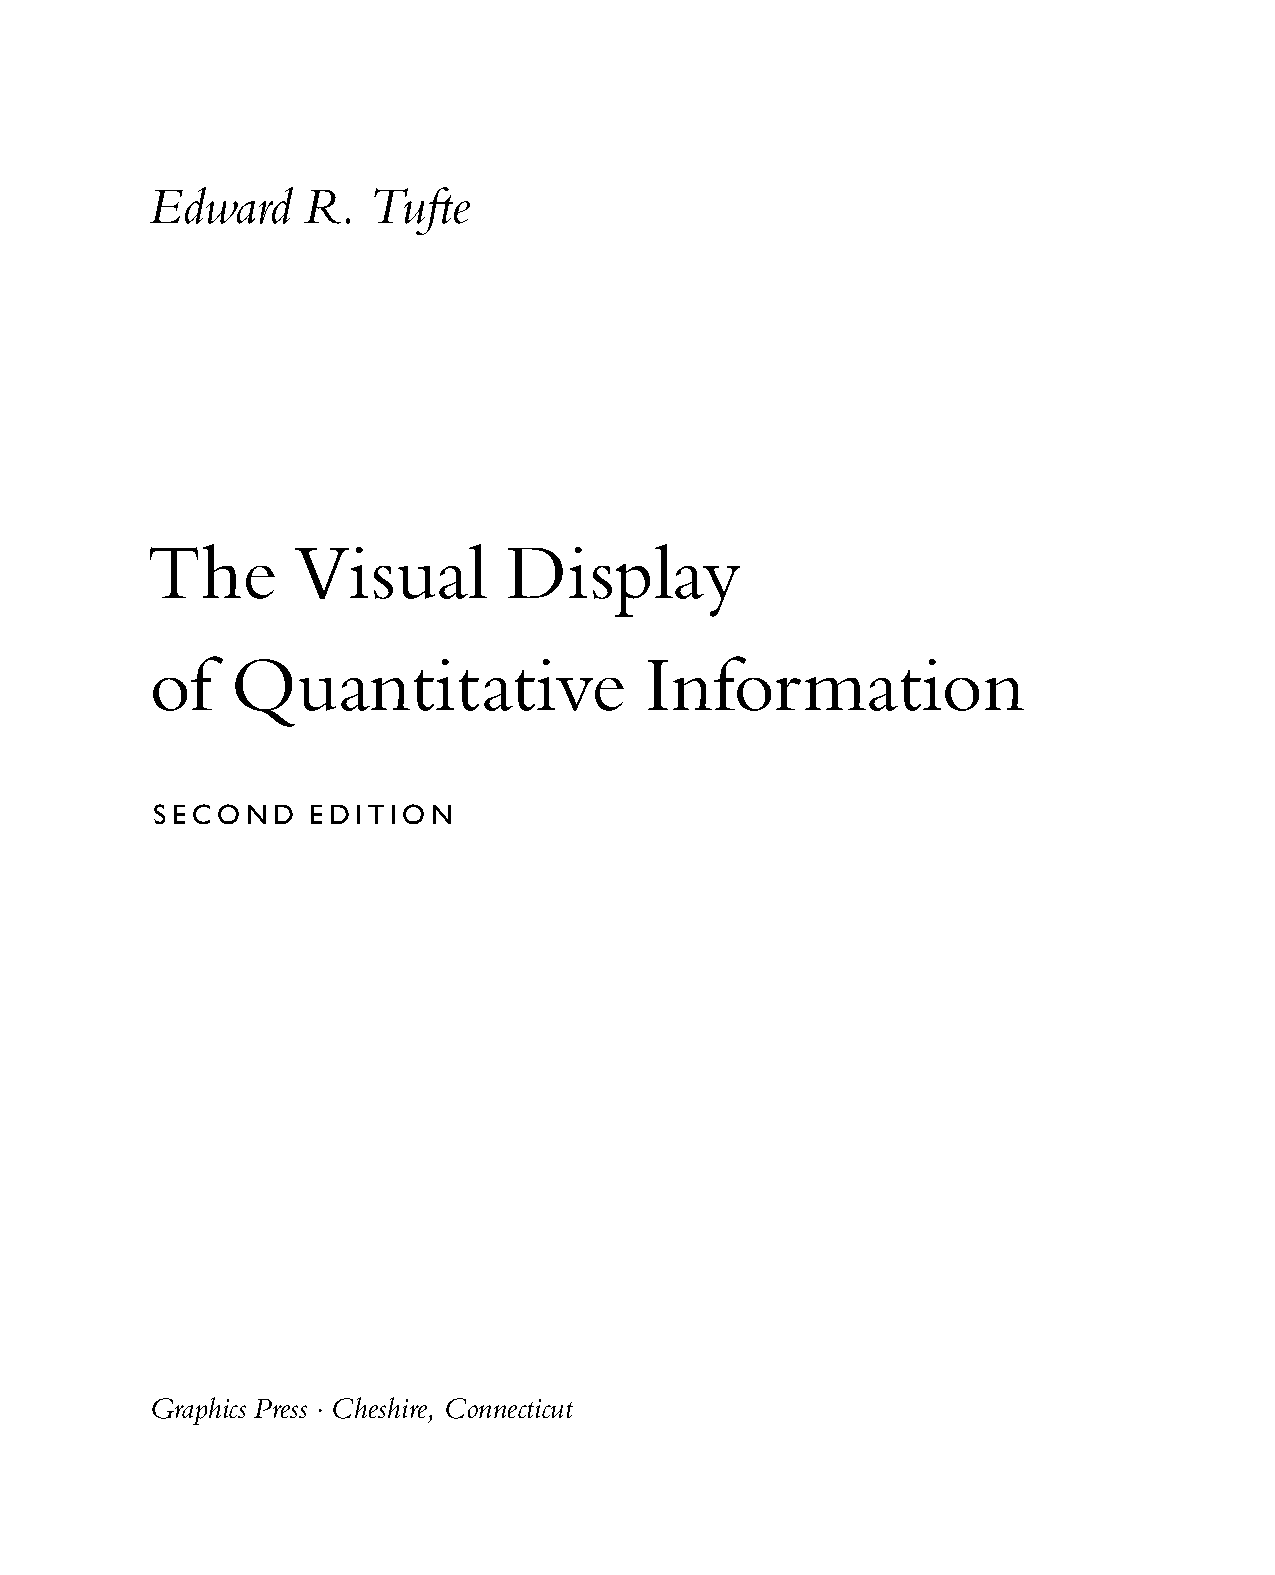
\includegraphics[width=0.45\linewidth]{figures/vdqi-title.pdf}}
\hfill
\fbox{
\includegraphics[width=0.45\linewidth]{figures/ei-title.pdf}}
\\\vspace{\baselineskip}
\fbox{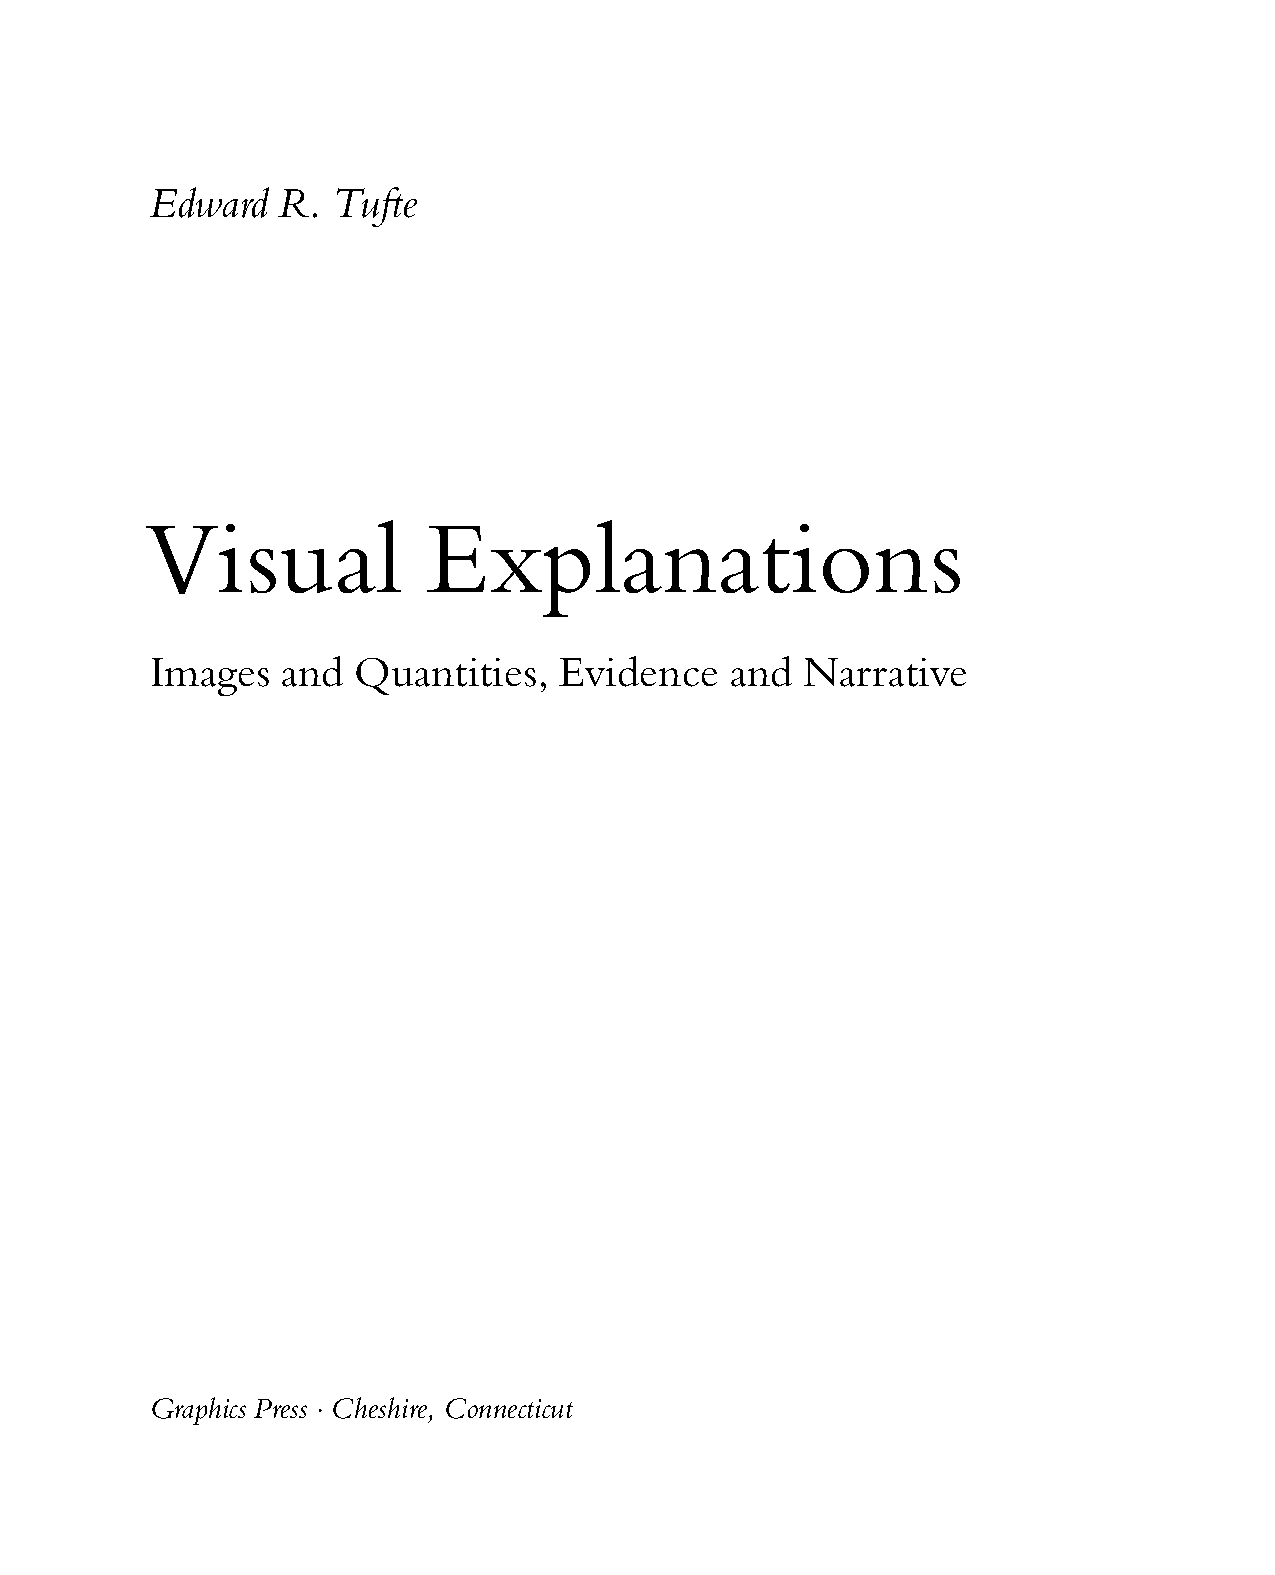
\includegraphics[width=0.45\linewidth]{figures/ve-title.pdf}}
\hfill
\fbox{
\includegraphics[width=0.45\linewidth]{figures/be-title.pdf}}
\end{figure*}

\newthought{The tables of contents} in Tufte's books give us our first
glimpse of the structure of the main matter. 
\begin{figure*}[p]\index{table of contents}
\fbox{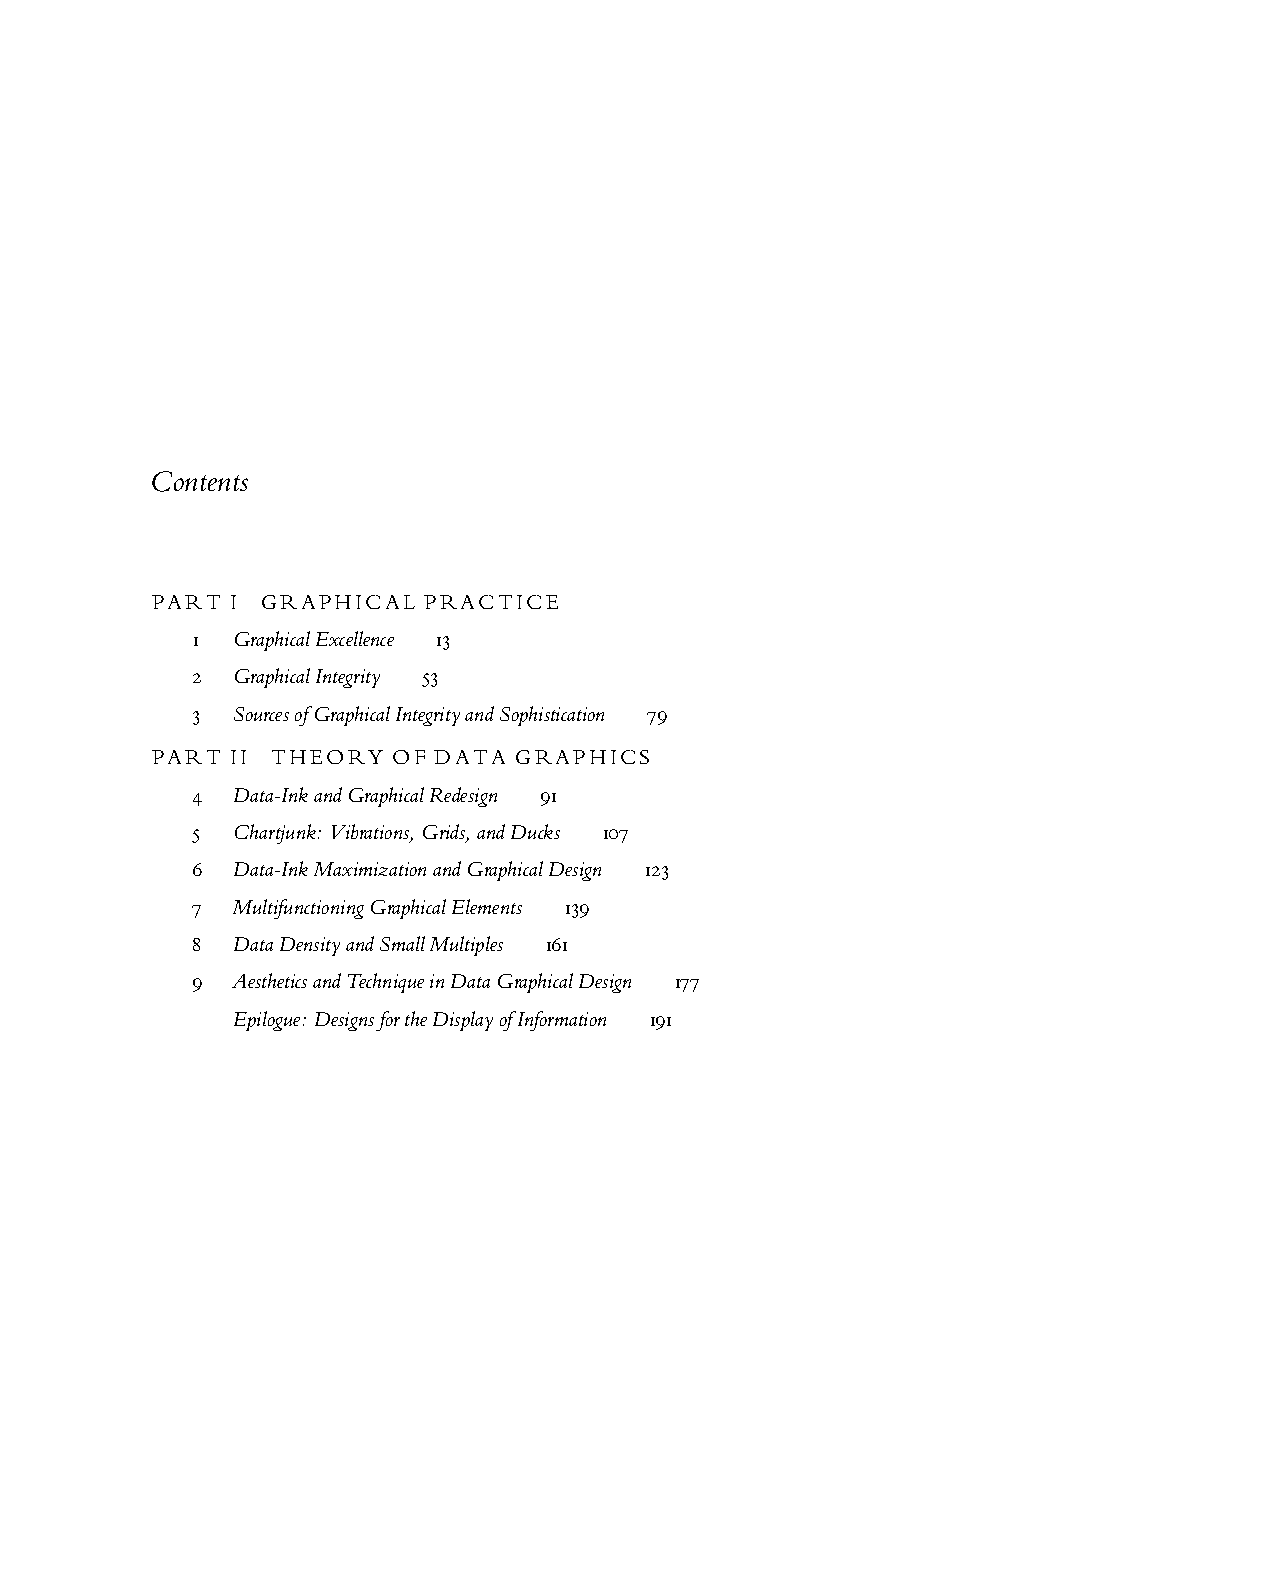
\includegraphics[width=0.45\linewidth]{figures/vdqi-contents.pdf}}
\hfill
\fbox{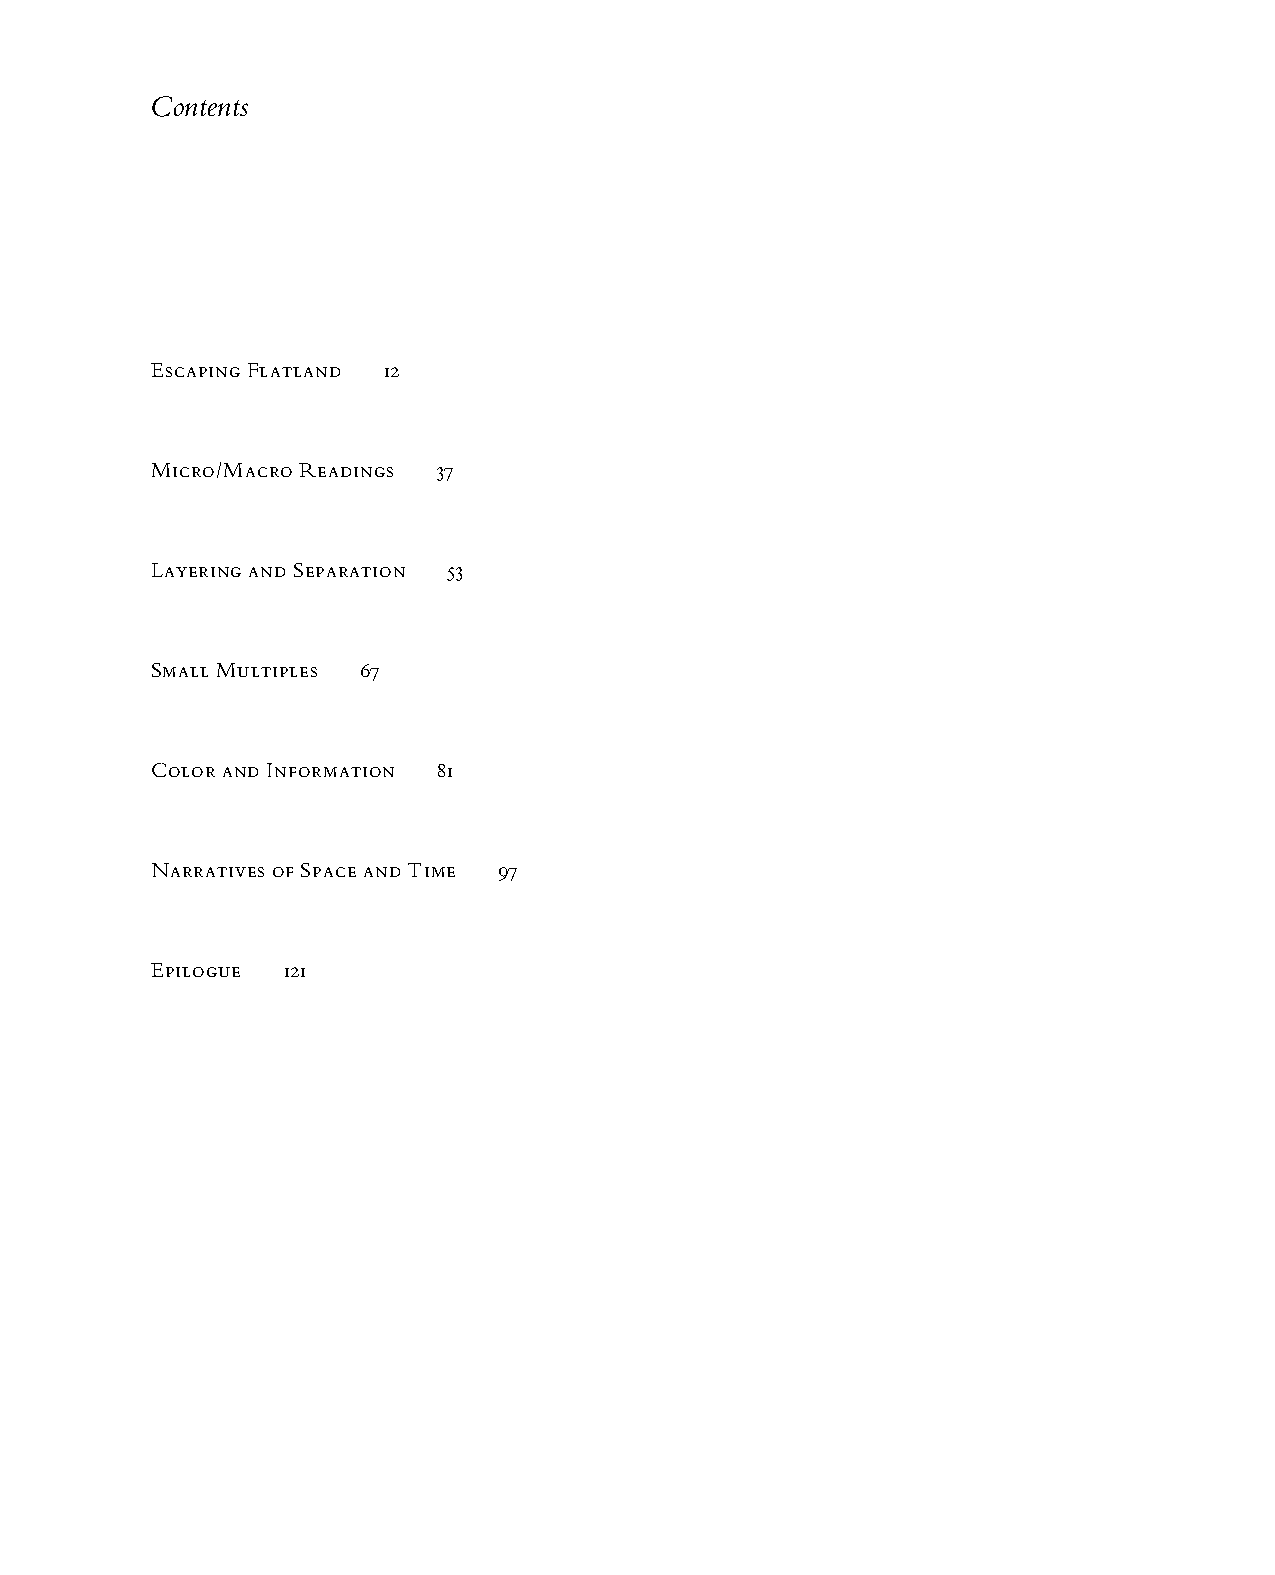
\includegraphics[width=0.45\linewidth]{figures/ei-contents.pdf}}
\\\vspace{\baselineskip}
\fbox{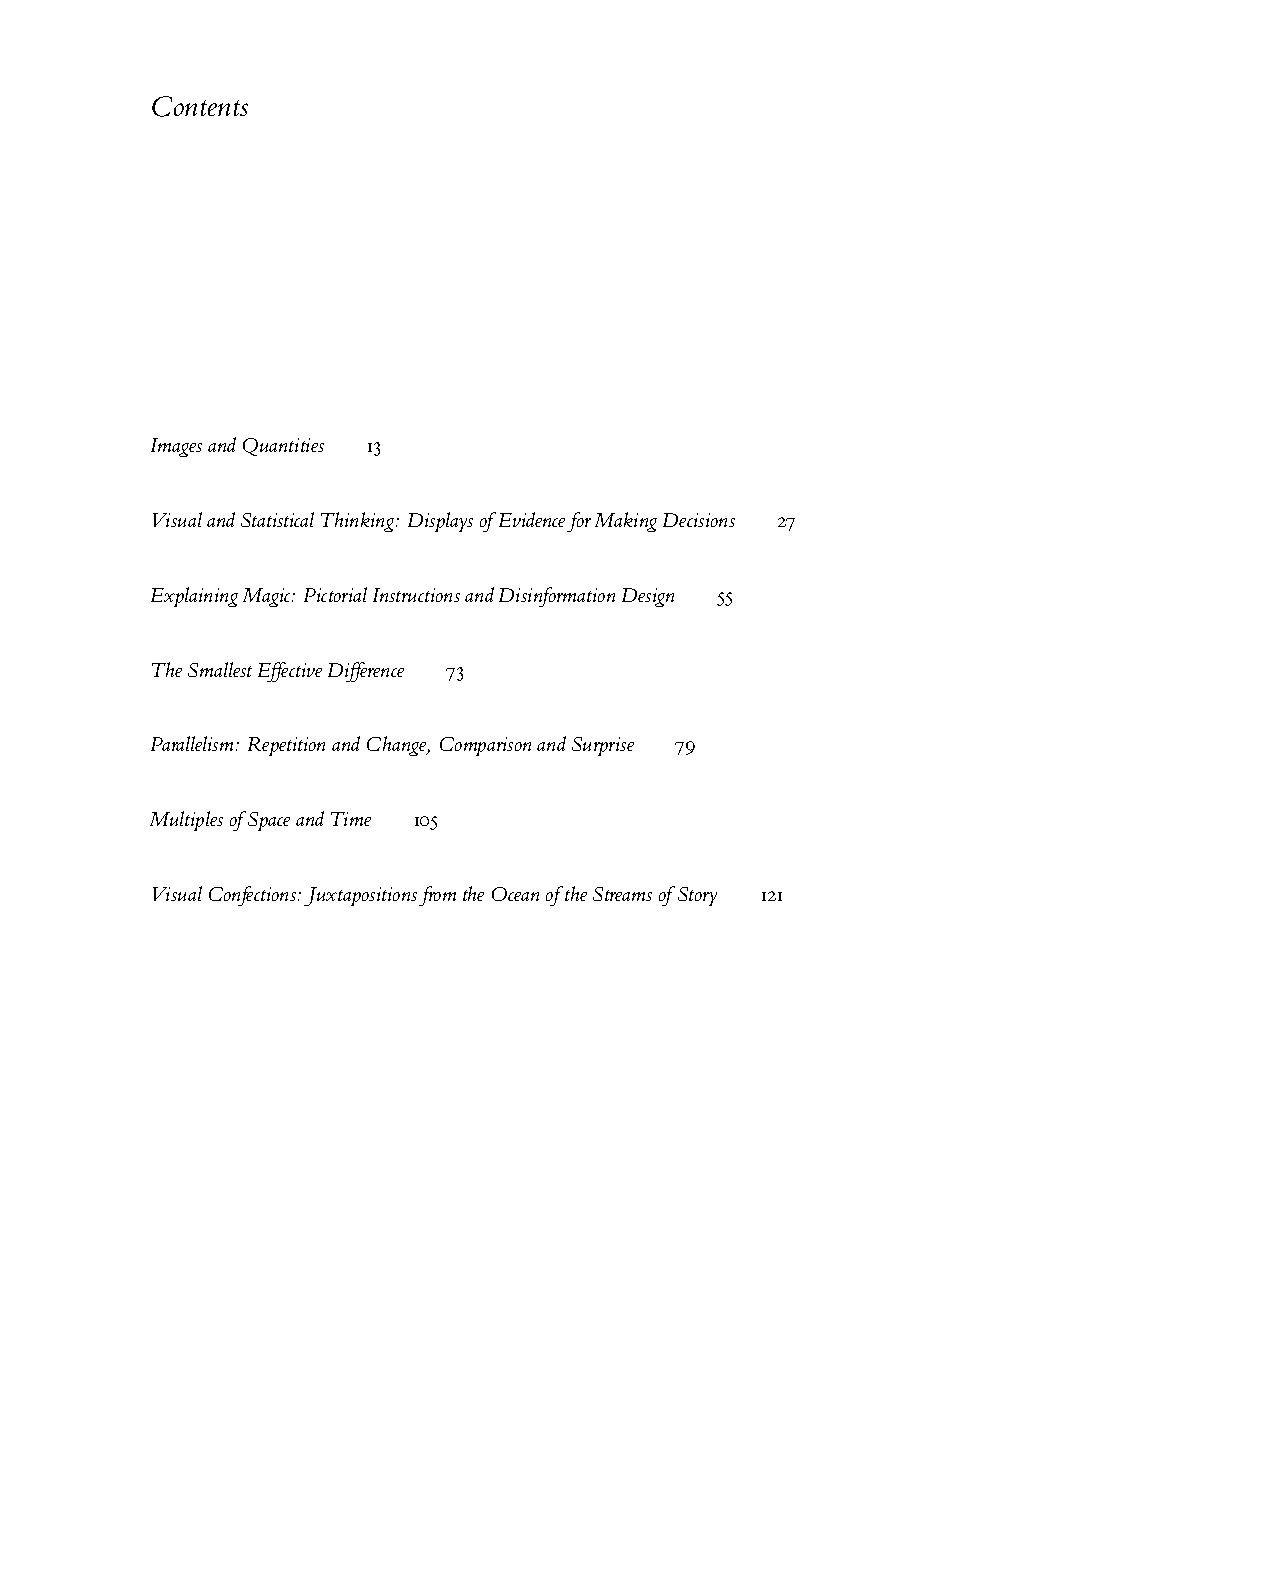
\includegraphics[width=0.45\linewidth]{figures/ve-contents.pdf}}
\hfill
\fbox{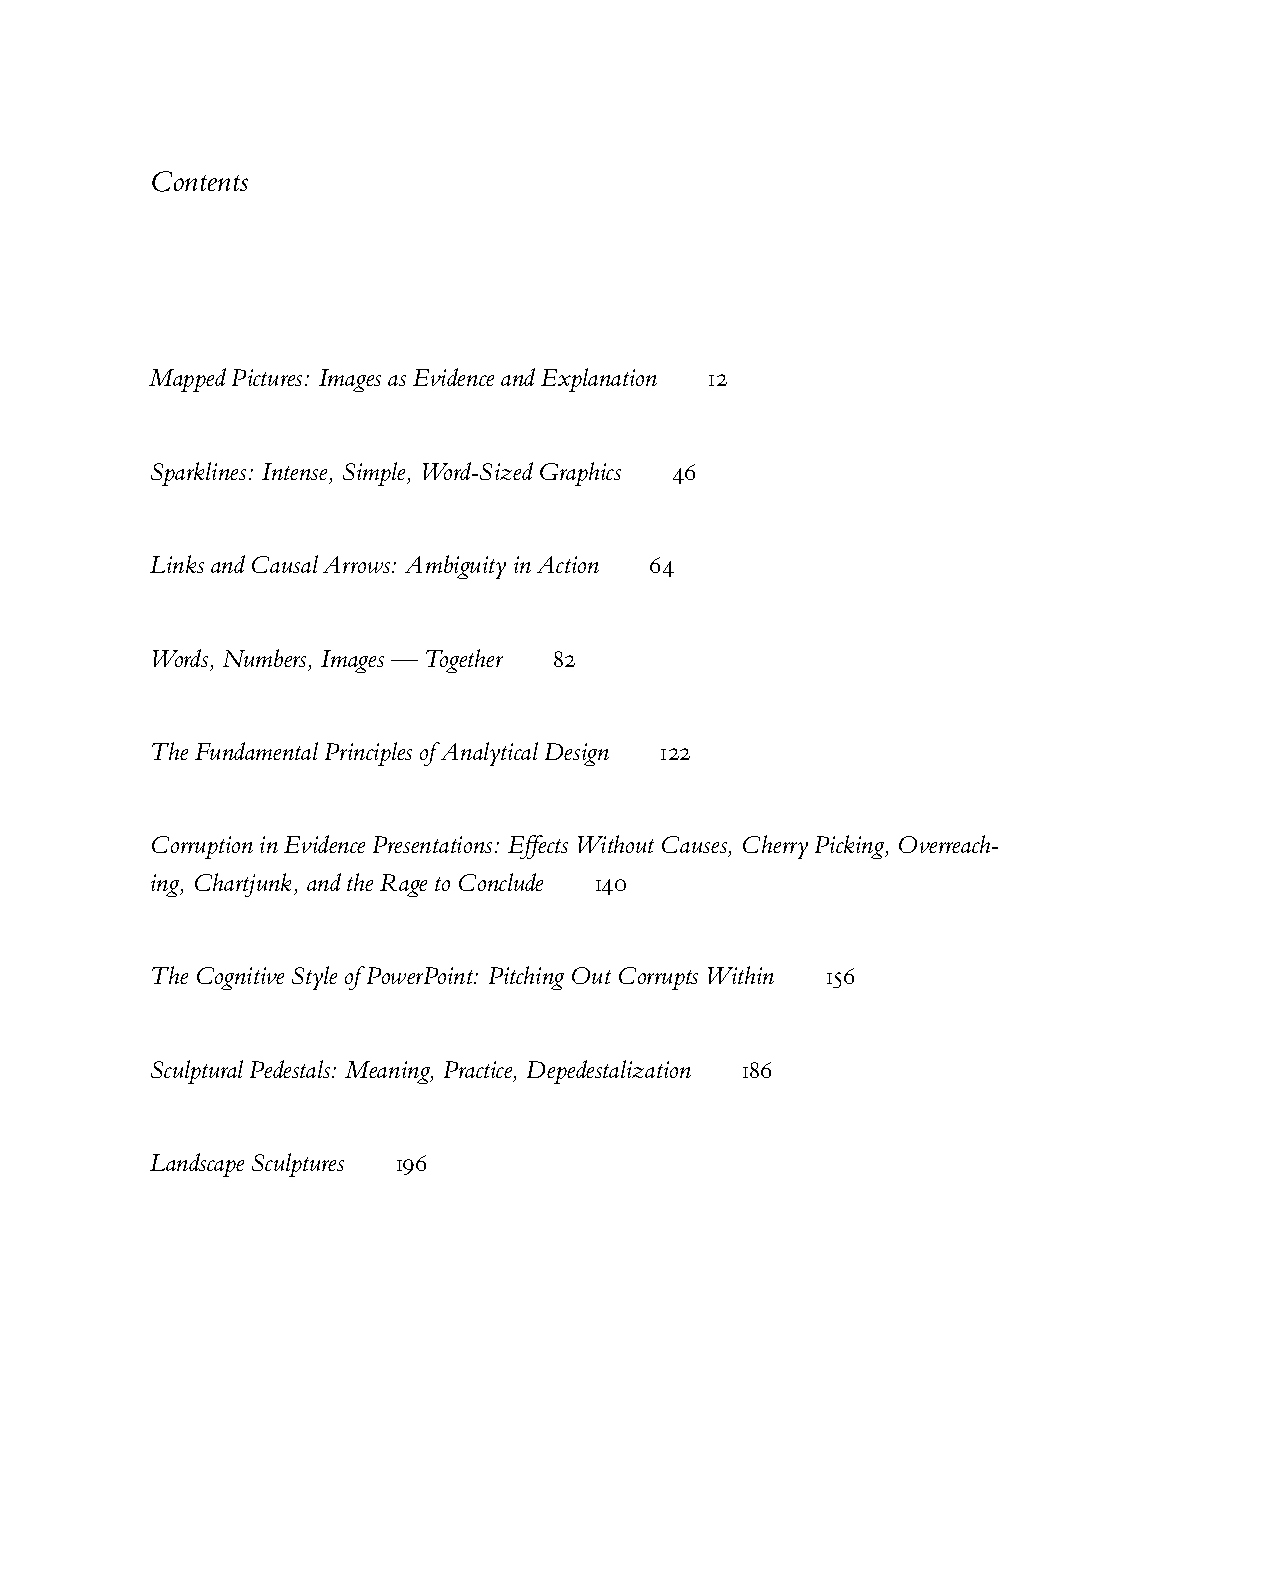
\includegraphics[width=0.45\linewidth]{figures/be-contents.pdf}}
\end{figure*}


\section{Headings}\label{sec:headings1}\index{headings}

Tufte's books include the following heading levels: parts,
chapters,\sidenote{Parts and chapters are defined for the \texttt{tufte-book}
class only.}  sections, subsections, and paragraphs.  Not defined by default
are: sub-subsections and subparagraphs.

\paragraph{Paragraph} Paragraph headings (as shown here) are introduced by
italicized text and separated from the main paragraph by a bit of space.

\section{Environments}

The following characteristics define the various environments:


\chapter[On the Use of the tufte-book Document Class]{On the Use of the \texttt{tufte-book} Document Class}
\label{ch:tufte-book}

Tufte's style is known
for its extensive use of sidenotes, tight integration of graphics with
text, and well-set typography.  This document aims to be at once a
demonstration of the features of the document classes
and a style guide to their use.

\section{Page Layout}\label{sec:page-layout}
\subsection{Headings}\label{sec:headings}\index{headings}
This style provides \textsc{a}- and \textsc{b}-heads (that is,
\Verb|\section| and \Verb|\subsection|), demonstrated above.

If you need more than two levels of section headings, you'll have to define
them yourself at the moment; there are no pre-defined styles for anything below
a \Verb|\subsection|.  As Bringhurst points out in \textit{The Elements of
Typographic Style},\cite{Bringhurst2005} you should ``use as many levels of
headings as you need: no more, and no fewer.''

The classes will emit an error if you try to use
\linebreak\Verb|\subsubsection| and smaller headings.

% let's start a new thought -- a new section
\newthought{In his later books},\cite{Tufte2006} Tufte
starts each section with a bit of vertical space, a non-indented paragraph,
and sets the first few words of the sentence in \textsc{small caps}.  To
accomplish this using this style, use the \doccmddef{newthought} command:
\begin{docspec}
  \doccmd{newthought}\{In his later books\}, Tufte starts\ldots
\end{docspec}


\section{Sidenotes}\label{sec:sidenotes}
One of the most prominent and distinctive features of this style is the
extensive use of sidenotes.  There is a wide margin to provide ample room
for sidenotes and small figures.  Any \doccmd{footnote}s will automatically
be converted to sidenotes.\footnote{This is a sidenote that was entered
using the \texttt{\textbackslash footnote} command.}  If you'd like to place ancillary
information in the margin without the sidenote mark (the superscript
number), you can use the \doccmd{marginnote} command.\marginnote{This is a
margin note.  Notice that there isn't a number preceding the note, and
there is no number in the main text where this note was written.}

The specification of the \doccmddef{sidenote} command is:
\begin{docspec}
  \doccmd{sidenote}[\docopt{number}][\docopt{offset}]\{\docarg{Sidenote text.}\}
\end{docspec}

Both the \docopt{number} and \docopt{offset} arguments are optional.  If you
provide a \docopt{number} argument, then that number will be used as the
sidenote number.  It will change the number of the current sidenote only and
will not affect the numbering sequence of subsequent sidenotes.

Sometimes a sidenote may run over the top of other text or graphics in the
margin space.  If this happens, you can adjust the vertical position of the
sidenote by providing a dimension in the \docopt{offset} argument.  Some
examples of valid dimensions are:
\begin{docspec}
  \ttfamily 1.0in \qquad 2.54cm \qquad 254mm \qquad 6\Verb|\baselineskip|
\end{docspec}
If the dimension is positive it will push the sidenote down the page; if the
dimension is negative, it will move the sidenote up the page.

While both the \docopt{number} and \docopt{offset} arguments are optional, they
must be provided in order.  To adjust the vertical position of the sidenote
while leaving the sidenote number alone, use the following syntax:
\begin{docspec}
  \doccmd{sidenote}[][\docopt{offset}]\{\docarg{Sidenote text.}\}
\end{docspec}
The empty brackets tell the \Verb|\sidenote| command to use the default
sidenote number.

If you \emph{only} want to change the sidenote number, however, you may
completely omit the \docopt{offset} argument:
\begin{docspec}
  \doccmd{sidenote}[\docopt{number}]\{\docarg{Sidenote text.}\}
\end{docspec}

The \doccmddef{marginnote} command has a similar \docarg{offset} argument:
\begin{docspec}
  \doccmd{marginnote}[\docopt{offset}]\{\docarg{Margin note text.}\}
\end{docspec}

\section{References}
References are placed alongside their citations as sidenotes,
as well.  This can be accomplished using the normal \doccmddef{cite}
command.\sidenote{The first paragraph of this document includes a citation.}

The complete list of references may also be printed automatically by using
the \doccmddef{bibliography} command.  (See the end of this document for an
example.)  If you do not want to print a bibliography at the end of your
document, use the \doccmddef{nobibliography} command in its place.  

To enter multiple citations at one location,\cite{Tufte2006,Tufte1990} you can
provide a list of keys separated by commas and the same optional vertical
offset argument: \Verb|\cite{Tufte2006,Tufte1990}|.  
\begin{docspec}
  \doccmd{cite}[\docopt{offset}]\{\docarg{bibkey1,bibkey2,\ldots}\}
\end{docspec}

\section{Figures and Tables}\label{sec:figures-and-tables}
Images and graphics play an integral role in Tufte's work.
In addition to the standard \docenvdef{figure} and \docenvdef{tabular} environments,
this style provides special figure and table environments for full-width
floats.

Full page--width figures and tables may be placed in \docenvdef{figure*} or
\docenvdef{table*} environments.  To place figures or tables in the margin,
use the \docenvdef{marginfigure} or \docenvdef{margintable} environments as follows
(see figure~\ref{fig:marginfig}):

\begin{marginfigure}%
  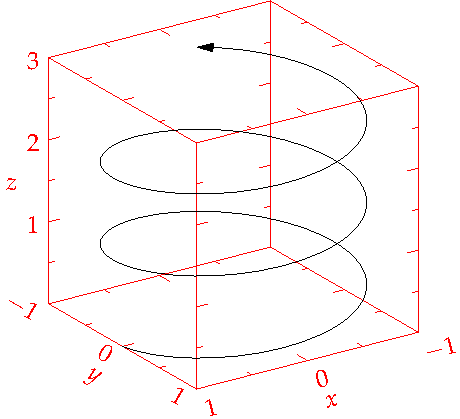
\includegraphics[width=\linewidth]{helix}
  \caption{This is a margin figure.  The helix is defined by 
    $x = \cos(2\pi z)$, $y = \sin(2\pi z)$, and $z = [0, 2.7]$.  The figure was
    drawn using Asymptote (\url{http://asymptote.sf.net/}).}
  \label{fig:marginfig}
\end{marginfigure}

\begin{docspec}
\textbackslash begin\{marginfigure\}\\
  \qquad\textbackslash includegraphics\{helix\}\\
  \qquad\textbackslash caption\{This is a margin figure.\}\\
  \qquad\textbackslash label\{fig:marginfig\}\\
\textbackslash end\{marginfigure\}\\
\end{docspec}

The \docenv{marginfigure} and \docenv{margintable} environments accept an optional parameter \docopt{offset} that adjusts the vertical position of the figure or table.  See the ``\nameref{sec:sidenotes}'' section above for examples.  The specifications are:
\begin{docspec}
  \textbackslash{begin\{marginfigure\}[\docopt{offset}]}\\
  \qquad\ldots\\
  \textbackslash{end\{marginfigure\}}\\
  \mbox{}\\
  \textbackslash{begin\{margintable\}[\docopt{offset}]}\\
  \qquad\ldots\\
  \textbackslash{end\{margintable\}}\\
\end{docspec}

Figure~\ref{fig:fullfig} is an example of the \docenv{figure*}
environment and figure~\ref{fig:textfig} is an example of the normal
\docenv{figure} environment.

\begin{figure*}[h]
  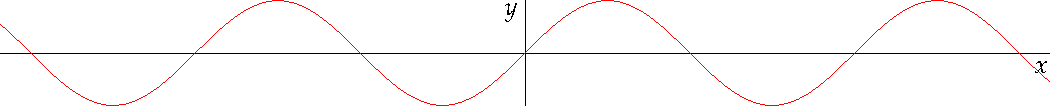
\includegraphics[width=\linewidth]{sine.pdf}%
  \caption{This graph shows $y = \sin x$ from about $x = [-10, 10]$.
  \emph{Notice that this figure takes up the full page width.}}%
  \label{fig:fullfig}%
\end{figure*}

\begin{figure}
  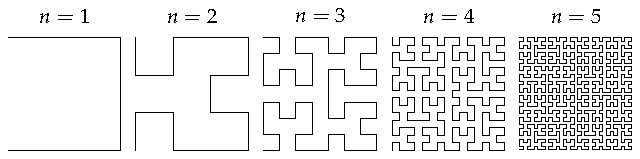
\includegraphics{hilbertcurves.pdf}
%  \checkparity This is an \pageparity\ page.%
  \caption[Hilbert curves of various degrees $n$.][6pt]{Hilbert curves of various degrees $n$. \emph{Notice that this figure only takes up the main textblock width.}}
  \label{fig:textfig}
  %\zsavepos{pos:textfig}
\end{figure}

As with sidenotes and marginnotes, a caption may sometimes require vertical
adjustment. The \doccmddef{caption} command now takes a second optional
argument that enables you to do this by providing a dimension \docopt{offset}.
You may specify the caption in any one of the following forms:
\begin{docspec}
  \doccmd{caption}\{\docarg{long caption}\}\\
  \doccmd{caption}[\docarg{short caption}]\{\docarg{long caption}\}\\
  \doccmd{caption}[][\docopt{offset}]\{\docarg{long caption}\}\\
  \doccmd{caption}[\docarg{short caption}][\docopt{offset}]%
                  \{\docarg{long caption}\}
\end{docspec}
A positive \docopt{offset} will push the caption down the page. The short
caption, if provided, is what appears in the list of figures/tables, otherwise
the ``long'' caption appears there. Note that although the arguments
\docopt{short caption} and \docopt{offset} are both optional, they must be
provided in order. Thus, to specify an \docopt{offset} without specifying a
\docopt{short caption}, you must include the first set of empty brackets
\Verb|[]|, which tell \doccmd{caption} to use the default ``long'' caption. As
an example, the caption to figure~\ref{fig:textfig} above was given in the form
\begin{docspec}
  \doccmd{caption}[Hilbert curves...][6pt]\{Hilbert curves...\}
\end{docspec}

Table~\ref{tab:normaltab} shows table created with the \docpkg{booktabs}
package.  Notice the lack of vertical rules---they serve only to clutter
the table's data.


\newthought{Occasionally} \LaTeX{} will generate an error message:\label{err:too-many-floats}
\begin{docspec}
  Error: Too many unprocessed floats
\end{docspec}
\LaTeX{} tries to place floats in the best position on the page.  Until it's
finished composing the page, however, it won't know where those positions are.
If you have a lot of floats on a page (including sidenotes, margin notes,
figures, tables, etc.), \LaTeX{} may run out of ``slots'' to keep track of them
and will generate the above error.

\LaTeX{} initially allocates 18 slots for storing floats.  To work around this
limitation, the document classes provide a \doccmddef{morefloats} command
that will reserve more slots.

The first time \doccmd{morefloats} is called, it allocates an additional 34
slots.  The second time \doccmd{morefloats} is called, it allocates another 26
slots.

The \doccmd{morefloats} command may only be used two times.  Calling it a
third time will generate an error message.  (This is because we can't safely
allocate many more floats or \LaTeX{} will run out of memory.)

If, after using the \doccmd{morefloats} command twice, you continue to get the
\texttt{Too many unprocessed floats} error, there are a couple things you can
do.

The \doccmddef{FloatBarrier} command will immediately process all the floats
before typesetting more material.  Since \doccmd{FloatBarrier} will start a new
paragraph, you should place this command at the beginning or end of a
paragraph.

The \doccmddef{clearpage} command will also process the floats before
continuing, but instead of starting a new paragraph, it will start a new page.

You can also try moving your floats around a bit: move a figure or table to the
next page or reduce the number of sidenotes.  (Each sidenote actually uses
\emph{two} slots.)

After the floats have placed, \LaTeX{} will mark those slots as unused so they
are available for the next page to be composed.

\section{Captions}
You may notice that the captions are sometimes misaligned.
Due to the way \LaTeX's float mechanism works, we can't know for sure where it
decided to put a float. Therefore, the document classes provide commands to
override the caption position.

\paragraph{Vertical alignment} To override the vertical alignment, use the
\doccmd{setfloatalignment} command inside the float environment.  For
example:

\begin{fullwidth}
\begin{docspec}
  \textbackslash begin\{figure\}[btp]\\
  \qquad \textbackslash includegraphics\{sinewave\}\\
  \qquad \textbackslash caption\{This is an example of a sine wave.\}\\
  \qquad \textbackslash label\{fig:sinewave\}\\
  \qquad \hlred{\textbackslash setfloatalignment\{b\}\% forces caption to be bottom-aligned}\\
  \textbackslash end\{figure\}
\end{docspec}
\end{fullwidth}

\noindent The syntax of the \doccmddef{setfloatalignment} command is:

\begin{docspec}
  \doccmd{setfloatalignment}\{\docopt{pos}\}
\end{docspec}

\noindent where \docopt{pos} can be either \texttt{b} for bottom-aligned
captions, or \texttt{t} for top-aligned captions.

\paragraph{Horizontal alignment}\label{par:overriding-horizontal}
To override the horizontal alignment, use either the \doccmd{forceversofloat}
or the \doccmd{forcerectofloat} command inside of the float environment.  For
example:

\begin{fullwidth}
\begin{docspec}
  \textbackslash begin\{figure\}[btp]\\
  \qquad \textbackslash includegraphics\{sinewave\}\\
  \qquad \textbackslash caption\{This is an example of a sine wave.\}\\
  \qquad \textbackslash label\{fig:sinewave\}\\
  \qquad \hlred{\textbackslash forceversofloat\% forces caption to be set to the left of the float}\\
  \textbackslash end\{figure\}
\end{docspec}
\end{fullwidth}

The \doccmddef{forceversofloat} command causes the algorithm to assume the
float has been placed on a verso page---that is, a page on the left side of a
two-page spread.  Conversely, the \doccmddef{forcerectofloat} command causes
the algorithm to assume the float has been placed on a recto page---that is, a
page on the right side of a two-page spread.


\section{Full-width text blocks}

In addition to the new float types, there is a \docenvdef{fullwidth}
environment that stretches across the main text block and the sidenotes
area.

\begin{Verbatim}
\begin{fullwidth}
Lorem ipsum dolor sit amet...
\end{fullwidth}
\end{Verbatim}

\begin{fullwidth}
The news and popular culture want us to fear the robot apocolypse.  Newspapers warn us that robots are coming for our jobs, and science fiction claims that the robots are coming for our lives.  At the same time, researchers building artificial intelligence are heralding their sucesses at Go,\cite{silver-16} Starcraft,\cite{vinyals2017starcraft} and Jeopardy!:\cite{ferruci-10} a revolution is around the corner.
\end{fullwidth}

\section{Typography}\label{sec:typography}

\subsection{Typefaces}\label{sec:typefaces}\index{typefaces}
If the Palatino, \textsf{Helvetica}, and \texttt{Bera Mono} typefaces are installed, this style
will use them automatically.  Otherwise, we'll fall back on the Computer Modern
typefaces.

\subsection{Letterspacing}\label{sec:letterspacing}
This document class includes two new commands and some improvements on
existing commands for letterspacing.

When setting strings of \allcaps{ALL CAPS} or \smallcaps{small caps}, the
letter\-spacing---that is, the spacing between the letters---should be
increased slightly.\cite{Bringhurst2005}  The \doccmddef{allcaps} command has proper letterspacing for
strings of \allcaps{FULL CAPITAL LETTERS}, and the \doccmddef{smallcaps} command
has letterspacing for \smallcaps{small capital letters}.  These commands
will also automatically convert the case of the text to upper- or
lowercase, respectively.

The \doccmddef{textsc} command has also been redefined to include
letterspacing.  The case of the \doccmd{textsc} argument is left as is,
however.  This allows one to use both uppercase and lowercase letters:
\textsc{The Initial Letters Of The Words In This Sentence Are Capitalized.}



\section{Document Class Options}\label{sec:options}

\index{class options|(}
The \doccls{tufte-book} class is based on the \LaTeX\ \doccls{book}
document class.  Therefore, you can pass any of the typical book
options.  There are a few options that are specific to the
\doccls{tufte-book} document class, however.

The \docclsoptdef{a4paper} option will set the paper size to \smallcaps{A4} instead of
the default \smallcaps{US} letter size.

The \docclsoptdef{sfsidenotes} option will set the sidenotes and title block in a 
\textsf{sans serif} typeface instead of the default roman.

The \docclsoptdef{twoside} option will modify the running heads so that the page
number is printed on the outside edge (as opposed to always printing the page
number on the right-side edge in \docclsoptdef{oneside} mode).  

The \docclsoptdef{symmetric} option typesets the sidenotes on the outside edge of
the page.  This is how books are traditionally printed, but is contrary to
Tufte's book design which sets the sidenotes on the right side of the page.
This option implicitly sets the \docclsopt{twoside} option.

The \docclsoptdef{justified} option sets all the text fully justified (flush left
and right).  The default is to set the text ragged right.  
The body text of Tufte's books are set ragged right.  This prevents
needless hyphenation and makes it easier to read the text in the slightly
narrower column.

The \docclsoptdef{bidi} option loads the \docpkg{bidi} package which is used with
\tXeLaTeX\ to typeset bi-directional text.  Since the \docpkg{bidi}
package needs to be loaded before the sidenotes and cite commands are defined,
it can't be loaded in the document preamble.

The \docclsoptdef{debug} option causes the classes to output debug
information to the log file which is useful in troubleshooting bugs.  It will
also cause the graphics to be replaced by outlines.

The \docclsoptdef{nofonts} option prevents the classes from
automatically loading the Palatino and Helvetica typefaces.  You should use
this option if you wish to load your own fonts.  If you're using \tXeLaTeX, this
option is implied (i.e., the Palatino and Helvetica fonts aren't loaded if you
use \tXeLaTeX).  

The \docclsoptdef{nols} option inhibits the letterspacing code.  The \TL\
classes try to load the appropriate letterspacing package (either pdf\TeX's
\docpkg{letterspace} package or the \docpkg{soul} package).  If you're using
\tXeLaTeX\ with \docpkg{fontenc}, however, you should configure your own
letterspacing.  

The \docclsoptdef{notitlepage} option causes \doccmd{maketitle} to generate a title
block instead of a title page.  The \doccls{book} class defaults to a title
page and the \doccls{handout} class defaults to the title block.  There is an
analogous \docclsoptdef{titlepage} option that forces \doccmd{maketitle} to
generate a full title page instead of the title block.

The \docclsoptdef{notoc} option suppresses \TL's custom table of contents
(\textsc{toc}) design.  The current \textsc{toc} design only shows unnumbered
chapter titles; it doesn't show sections or subsections.  The \docclsopt{notoc}
option will revert to \LaTeX's \textsc{toc} design.

The \docclsoptdef{nohyper} option prevents the \docpkg{hyperref} package from
being loaded.  The default is to load the \docpkg{hyperref} package and use the
\doccmd{title} and \doccmd{author} contents as metadata for the generated
\textsc{pdf}.

\index{class options|)}



\chapter[Customizing Tufte-LaTeX]{Customizing \TL}
\label{ch:customizing}

The document classes are designed to closely emulate Tufte's book
design by default.  However, each document is different and you may encounter
situations where the default settings are insufficient.  This chapter explores
many of the ways you can adjust the document classes to better fit
your needs.

\section{File Hooks}
\label{sec:filehooks}

\index{file hooks|(}
If you create many documents using the classes, it's easier to
store your customizations in a separate file instead of copying them into the
preamble of each document.  The classes provide three file hooks:
\docfilehook{tufte-common-local.tex}{common}, \docfilehook{tufte-book-local.tex}{book}, and
\docfilehook{tufte-handout-local.tex}{handout}.\sloppy

\begin{description}
  \item[\docfilehook{tufte-common-local.tex}{common}]
    If this file exists, it will be loaded by all of the document
    classes just prior to any document-class-specific code.  If your
    customizations or code should be included in both the book and handout
    classes, use this file hook.
  \item[\docfilehook{tufte-book-local.tex}{book}] 
    If this file exists, it will be loaded after all of the common and
    book-specific code has been read.  If your customizations apply only to the
    book class, use this file hook.
  \item[\docfilehook{tufte-common-handout.tex}{handout}] 
    If this file exists, it will be loaded after all of the common and
    handout-specific code has been read.  If your customizations apply only to
    the handout class, use this file hook.
\end{description}

\index{file hooks|)}

\section{Numbered Section Headings}
\label{sec:numbered-sections}
\index{headings!numbered}

While Tufte dispenses with numbered headings in his books, if you require them,
they can be anabled by changing the value of the \doccounter{secnumdepth}
counter.  From the table below, select the heading level at which numbering
should stop and set the \doccounter{secnumdepth} counter to that value.  For
example, if you want parts and chapters numbered, but don't want numbering for
sections or subsections, use the command:
\begin{docspec}
  \doccmd{setcounter}\{secnumdepth\}\{0\}
\end{docspec}

The default \doccounter{secnumdepth} for the document classes is $-1$.

\begin{table}
  \footnotesize
  \begin{center}
    \begin{tabular}{lr}
      \toprule
      Heading level & Value \\
      \midrule
      Part (in \doccls{tufte-book}) & $-1$ \\
      Part (in \doccls{tufte-handout}) & $0$ \\
      Chapter (only in \doccls{tufte-book}) & $0$ \\
      Section & $1$ \\
      Subsection & $2$ \\
      Subsubsection & $3$ \\
      Paragraph & $4$ \\
      Subparagraph & $5$ \\
      \bottomrule
    \end{tabular}
  \end{center}
  \caption{Heading levels used with the \texttt{secnumdepth} counter.}
\end{table}

\section{Changing the Paper Size}
\label{sec:paper-size}

The classes currently only provide three paper sizes: \textsc{a4},
\textsc{b5}, and \textsc{us} letter.  To specify a different paper size (and/or
margins), use the \doccmd[geometry]{geometry} command in the preamble of your
document (or one of the file hooks).  The full documentation of the
\doccmd{geometry} command may be found in the \docpkg{geometry} package
documentation.\cite{pkg-geometry}


\section{Customizing Marginal Material}
\label{sec:marginal-material}

Marginal material includes sidenotes, citations, margin notes, and captions.
Normally, the justification of the marginal material follows the justification
of the body text.  If you specify the \docclsopt{justified} document class
option, all of the margin material will be fully justified as well.  If you
don't specify the \docclsopt{justified} option, then the marginal material will
be set ragged right.

You can set the justification of the marginal material separately from the body
text using the following document class options: \docclsopt{sidenote},
\docclsopt{marginnote}, \docclsopt{caption}, \docclsopt{citation}, and
\docclsopt{marginals}.  Each option refers to its obviously corresponding
marginal material type.  The \docclsopt{marginals} option simultaneously sets
the justification on all four marginal material types.

Each of the document class options takes one of five justification types:
\begin{description}
  \item[\docclsopt{justified}] Fully justifies the text (sets it flush left and
    right).
  \item[\docclsopt{raggedleft}] Sets the text ragged left, regardless of which
    page it falls on.
  \item[\docclsopt{raggedright}] Sets the text ragged right, regardless of
    which page it falls on.
  \item[\doccls{raggedouter}] Sets the text ragged left if it falls on the
    left-hand (verso) page of the spread and otherwise sets it ragged right.
    This is useful in conjunction with the \docclsopt{symmetric} document class
    option.
  \item[\docclsopt{auto}] If the \docclsopt{justified} document class option
    was specified, then set the text fully justified; otherwise the text is set
    ragged right.  This is the default justification option if one is not
    explicitly specified.
\end{description}

\noindent For example, 
\begin{docspec}
  \doccmdnoindex{documentclass}[symmetric,justified,marginals=raggedouter]\{tufte-book\}
\end{docspec}
will set the body text of the document to be fully justified and all of the
margin material (sidenotes, margin notes, captions, and citations) to be flush
against the body text with ragged outer edges.

\newthought{The font and style} of the marginal material may also be modified using the following commands:

\begin{docspec}
  \doccmd{setsidenotefont}\{\docopt{font commands}\}\\
  \doccmd{setcaptionfont}\{\docopt{font commands}\}\\
  \doccmd{setmarginnotefont}\{\docopt{font commands}\}\\
  \doccmd{setcitationfont}\{\docopt{font commands}\}
\end{docspec}

The \doccmddef{setsidenotefont} sets the font and style for sidenotes, the
\doccmddef{setcaptionfont} for captions, the \doccmddef{setmarginnotefont} for
margin notes, and the \doccmddef{setcitationfont} for citations.  The
\docopt{font commands} can contain font size changes (e.g.,
\doccmdnoindex{footnotesize}, \doccmdnoindex{Huge}, etc.), font style changes (e.g.,
\doccmdnoindex{sffamily}, \doccmdnoindex{ttfamily}, \doccmdnoindex{itshape}, etc.), color changes (e.g.,
\doccmdnoindex{color}\texttt{\{blue\}}), and many other adjustments.

If, for example, you wanted the captions to be set in italic sans serif, you could use:
\begin{docspec}
  \doccmd{setcaptionfont}\{\doccmdnoindex{itshape}\doccmdnoindex{sffamily}\}
\end{docspec}


%%
% The back matter contains appendices, bibliographies, indices, glossaries, etc.





\newcommand{\outline}[3]{\chapter{#1}
  \begin{itemize}
  \item {\bf Story:} #1
  \item {\bf Essay:} #2
  \end{itemize}
}

\outline{General AI}{\lastname{} is called in to consult on the
  deployment of a general AI that a military contractor has developed.
  It breaks out of its sandbox, causing physical havoc with military
  equipment.  A specialized AI designed to contain the general AI is
  surgically deployed to resolve the problem.}{This chapter explores
  the distinction between general and specialized
  AI---\specializedai{}---and how the pressures and history of a
  general AI cause them to be vulnerable to specialized algorithms and
  methods.}

\outline{Resource-Constrained AI}{\lastname{} is comfortably faculty
  at University when her past history with \specializedai{} comes back
  to haunt her: a rogue actor has found an old copy and using it to
  terrorize a small Canadian town.  \lastname{} works with the local
  authorities to deploy their specialized AI to counteract the
  threat.}{This chapter explores how governments' role as a protector
  of populations and evolves in a world with ubiquitous and powerful
  artifcial intelligence.  Although in some ways AI is democratizing,
  it is still connected to access to real-world resources (material,
  energy, physical space), and governments and multinational
  corporations will have the most powerful and capable AI agents.
  Just as we trust governments with technology that can end the world
  (nuclear weapons), we must trust the government to responsibly
  harness the power of artificial intelligence.}

\outline{AI's role in social interactions}{\lastname{} finds herself
  drawn into a political scandal when an AI agent begins influencing
  public opinion against her and her research.  She fights back the
  only way she knows how: with AI.}{While the threat of AI is often
  seen as physical, another salient fear is social and emotional: AIs
  can play on fear and emotion.  In many ways this is harder to notice
  and fight against because these effects might be superficially
  welcome by their targets.  This chapter talks about how AIs can
  detect, influence, and interact with people.}

\jbgcomment{Not putting in outline, but what might be a way of making
  the plot work, this could be a scheme by a faculty adversary that
  she uncovers, which leads her to sell out.}

\outline{Cashing Out}{Fed up by politics and the politics of academia,
  \lastname{} goes off to make a pile of money at \fintech{}, turning
  her AI smarts to Wall Street.  It's harder than she
  thinks.}{Financial markets, like much of AI, hope to make
  predictions about what will happen in the world and to estimate
  uncertainty.  This chapter investigates whether capitalist markets
  is possible in a world with effective AI.}

\jbgcomment{Connection between the two chapters: previous chapter allows everyone to go out an earn a capitalist wage.}

\outline{The Silent Revolution}{Having saved the world multiple times,
  \lastname{} retires to spend more time with her grandchildren and
  sees their relationship with AI.}{The book concludes with how AI can
  change social interactions and society in less overtly negative
  ways, warning about a future where AI can diminish the richness of
  the human experience (if we let it).}

\backmatter

\bibliography{bib/jbg}
\bibliographystyle{plainnat}


\printindex

\end{document}
